% Options for packages loaded elsewhere
\PassOptionsToPackage{unicode}{hyperref}
\PassOptionsToPackage{hyphens}{url}
%
\documentclass[
]{article}
\usepackage{lmodern}
\usepackage{amssymb,amsmath}
\usepackage{ifxetex,ifluatex}
\ifnum 0\ifxetex 1\fi\ifluatex 1\fi=0 % if pdftex
  \usepackage[T1]{fontenc}
  \usepackage[utf8]{inputenc}
  \usepackage{textcomp} % provide euro and other symbols
\else % if luatex or xetex
  \usepackage{unicode-math}
  \defaultfontfeatures{Scale=MatchLowercase}
  \defaultfontfeatures[\rmfamily]{Ligatures=TeX,Scale=1}
\fi
% Use upquote if available, for straight quotes in verbatim environments
\IfFileExists{upquote.sty}{\usepackage{upquote}}{}
\IfFileExists{microtype.sty}{% use microtype if available
  \usepackage[]{microtype}
  \UseMicrotypeSet[protrusion]{basicmath} % disable protrusion for tt fonts
}{}
\makeatletter
\@ifundefined{KOMAClassName}{% if non-KOMA class
  \IfFileExists{parskip.sty}{%
    \usepackage{parskip}
  }{% else
    \setlength{\parindent}{0pt}
    \setlength{\parskip}{6pt plus 2pt minus 1pt}}
}{% if KOMA class
  \KOMAoptions{parskip=half}}
\makeatother
\usepackage{xcolor}
\IfFileExists{xurl.sty}{\usepackage{xurl}}{} % add URL line breaks if available
\IfFileExists{bookmark.sty}{\usepackage{bookmark}}{\usepackage{hyperref}}
\hypersetup{
  pdftitle={DEM 7223 - Event History Analysis - Parametric Hazard Models},
  hidelinks,
  pdfcreator={LaTeX via pandoc}}
\urlstyle{same} % disable monospaced font for URLs
\usepackage[margin=1in]{geometry}
\usepackage{color}
\usepackage{fancyvrb}
\newcommand{\VerbBar}{|}
\newcommand{\VERB}{\Verb[commandchars=\\\{\}]}
\DefineVerbatimEnvironment{Highlighting}{Verbatim}{commandchars=\\\{\}}
% Add ',fontsize=\small' for more characters per line
\usepackage{framed}
\definecolor{shadecolor}{RGB}{248,248,248}
\newenvironment{Shaded}{\begin{snugshade}}{\end{snugshade}}
\newcommand{\AlertTok}[1]{\textcolor[rgb]{0.94,0.16,0.16}{#1}}
\newcommand{\AnnotationTok}[1]{\textcolor[rgb]{0.56,0.35,0.01}{\textbf{\textit{#1}}}}
\newcommand{\AttributeTok}[1]{\textcolor[rgb]{0.77,0.63,0.00}{#1}}
\newcommand{\BaseNTok}[1]{\textcolor[rgb]{0.00,0.00,0.81}{#1}}
\newcommand{\BuiltInTok}[1]{#1}
\newcommand{\CharTok}[1]{\textcolor[rgb]{0.31,0.60,0.02}{#1}}
\newcommand{\CommentTok}[1]{\textcolor[rgb]{0.56,0.35,0.01}{\textit{#1}}}
\newcommand{\CommentVarTok}[1]{\textcolor[rgb]{0.56,0.35,0.01}{\textbf{\textit{#1}}}}
\newcommand{\ConstantTok}[1]{\textcolor[rgb]{0.00,0.00,0.00}{#1}}
\newcommand{\ControlFlowTok}[1]{\textcolor[rgb]{0.13,0.29,0.53}{\textbf{#1}}}
\newcommand{\DataTypeTok}[1]{\textcolor[rgb]{0.13,0.29,0.53}{#1}}
\newcommand{\DecValTok}[1]{\textcolor[rgb]{0.00,0.00,0.81}{#1}}
\newcommand{\DocumentationTok}[1]{\textcolor[rgb]{0.56,0.35,0.01}{\textbf{\textit{#1}}}}
\newcommand{\ErrorTok}[1]{\textcolor[rgb]{0.64,0.00,0.00}{\textbf{#1}}}
\newcommand{\ExtensionTok}[1]{#1}
\newcommand{\FloatTok}[1]{\textcolor[rgb]{0.00,0.00,0.81}{#1}}
\newcommand{\FunctionTok}[1]{\textcolor[rgb]{0.00,0.00,0.00}{#1}}
\newcommand{\ImportTok}[1]{#1}
\newcommand{\InformationTok}[1]{\textcolor[rgb]{0.56,0.35,0.01}{\textbf{\textit{#1}}}}
\newcommand{\KeywordTok}[1]{\textcolor[rgb]{0.13,0.29,0.53}{\textbf{#1}}}
\newcommand{\NormalTok}[1]{#1}
\newcommand{\OperatorTok}[1]{\textcolor[rgb]{0.81,0.36,0.00}{\textbf{#1}}}
\newcommand{\OtherTok}[1]{\textcolor[rgb]{0.56,0.35,0.01}{#1}}
\newcommand{\PreprocessorTok}[1]{\textcolor[rgb]{0.56,0.35,0.01}{\textit{#1}}}
\newcommand{\RegionMarkerTok}[1]{#1}
\newcommand{\SpecialCharTok}[1]{\textcolor[rgb]{0.00,0.00,0.00}{#1}}
\newcommand{\SpecialStringTok}[1]{\textcolor[rgb]{0.31,0.60,0.02}{#1}}
\newcommand{\StringTok}[1]{\textcolor[rgb]{0.31,0.60,0.02}{#1}}
\newcommand{\VariableTok}[1]{\textcolor[rgb]{0.00,0.00,0.00}{#1}}
\newcommand{\VerbatimStringTok}[1]{\textcolor[rgb]{0.31,0.60,0.02}{#1}}
\newcommand{\WarningTok}[1]{\textcolor[rgb]{0.56,0.35,0.01}{\textbf{\textit{#1}}}}
\usepackage{graphicx,grffile}
\makeatletter
\def\maxwidth{\ifdim\Gin@nat@width>\linewidth\linewidth\else\Gin@nat@width\fi}
\def\maxheight{\ifdim\Gin@nat@height>\textheight\textheight\else\Gin@nat@height\fi}
\makeatother
% Scale images if necessary, so that they will not overflow the page
% margins by default, and it is still possible to overwrite the defaults
% using explicit options in \includegraphics[width, height, ...]{}
\setkeys{Gin}{width=\maxwidth,height=\maxheight,keepaspectratio}
% Set default figure placement to htbp
\makeatletter
\def\fps@figure{htbp}
\makeatother
\setlength{\emergencystretch}{3em} % prevent overfull lines
\providecommand{\tightlist}{%
  \setlength{\itemsep}{0pt}\setlength{\parskip}{0pt}}
\setcounter{secnumdepth}{-\maxdimen} % remove section numbering

\title{DEM 7223 - Event History Analysis - Parametric Hazard Models}
\author{true}
\date{September 21, 2020}

\begin{document}
\maketitle

{
\setcounter{tocdepth}{2}
\tableofcontents
}
\hypertarget{regression-modeling-of-duration-data}{%
\subsection{Regression modeling of duration
data}\label{regression-modeling-of-duration-data}}

\begin{itemize}
\item
  Up until now we have not been concerned with the effects of individual
  characteristics on the risk of experiencing an event.
\item
  We did see earlier that we can express the risk of experiencing an
  event conditional on individual risk factors, or covariates.
\item
  We first discuss the use of parametric models for doing this
\end{itemize}

\hypertarget{parametric-models}{%
\subsubsection{Parametric models}\label{parametric-models}}

\begin{itemize}
\item
  When we consider a parametric model in hazards analysis, we are saying
  that we intend to explicitly define the fundamental shape of our
  \emph{hazard function}, or that we are assuming a specific
  distribution for our durations.
\item
  If we make a poor assumption on either of these points, our analysis
  is often incorrect, because we have effectively defined the wrong
  model.
\item
  This is bad because our parameters that we think are telling us
  something, really are telling us nothing.
\item
  We've seen this concept before when considering the \emph{Generalized
  Linear Model} vs the \emph{Linear Model}. i.e.~Don't us the linear
  model for a binary outcome
\item
  We can use regression models for duration data in two ways:
\end{itemize}

\textbf{Proportional Hazards Model (PH)}

\[h(t_i) = h_0 \text{ } g(x_i)\] usually letting
\(g(x_i) = \text{exp } (x_i ' \beta)\)

\textbf{Accelerated Failure Time Model (AFT)}

\[log(t_i) = x_i ' \beta +z_i\]

letting \(z_i\) have a parametric density

\hypertarget{which-model-form-to-use}{%
\subsubsection{Which model form to use?}\label{which-model-form-to-use}}

What is being modeled? Hazard or time?

\begin{itemize}
\item
  In a proportional hazard model if a \(\beta >0\) it says that the
  hazard increases, if a \(\beta <0\) it says that the hazard decreases.
\item
  This is different than we are used to seeing for other regression
  models
\item
  If the hazard is higher, then the risk is greater. This implies that
  subjects experience the event at a faster rate, and on average the
  durations are shorter.
\end{itemize}

In a accelerated failure time model if a \(\beta >0\) it says that the
time, or duration increases, if a \(\beta <0\) it says that the time, or
duration decreases.

This is similar to what we are used to seeing for other regression
models.

\hypertarget{parameters-and-distributions}{%
\subsubsection{Parameters and
distributions}\label{parameters-and-distributions}}

Parameters are unknown quantities that we estimate from data.

They define characteristics of mathematical functions, and variations in
said functions.

Some examples of parametric models:

Linear regression, using the Normal distribution\\
\[y \sim Normal (b_0+b_1*x, \sigma^2_e)\] has 2 parameters, the mean,
here shown as the linear mean function, and the variance in the
residuals

Logistic regression has mean function that is a transform of the mean

\[y \sim Binomial \left ( \frac{1}{1+exp^{(b_0+b_1*x)} } \right)\]

In both of these models, we estimate the parameters, \(b_0\) and \(b_1\)
to describe how x affects y

In Parametric hazard models, we estimate regression parameters as well,
but we also estimate parameters that describe the \emph{shape of the
distribution} of duration times

E.g. the normal distribution function is defined by 2 parameters:
\(\mu\) and \(\sigma\), which define the characteristic bell-shaped
curve

\hypertarget{common-distributions-in-event-history-analysis}{%
\subsubsection{Common distributions in event history
analysis}\label{common-distributions-in-event-history-analysis}}

\begin{itemize}
\tightlist
\item
  Exponential This is a 1 parameter distribution, the hazard model for
  this is:
\end{itemize}

\[h_i(t,x_i) = h_0 \text{ } exp(x'\beta)\] The exponential is often a
starting point that we don't use very much. The biggest reason we don't
use it is because the hazard function is assumed to be a constant
(\(h_0\) isn't a function of time)

\begin{itemize}
\tightlist
\item
  Weibull The Weibull is a two parameter distribution, it's hazard
  function without covariates is:
\end{itemize}

\[h_i(t) = \theta \gamma t^{\gamma-1}\]

it's hazard function with covariates is:

\[h_i(t,x_i) = \gamma exp(x'\beta) t^{\gamma-1}\] You notice that
\(\theta\) is replaced with the mean function in the second equation.
The Weibull is a much more flexible distribution, and the shape of the
hazard function change as \(\gamma\) changes.

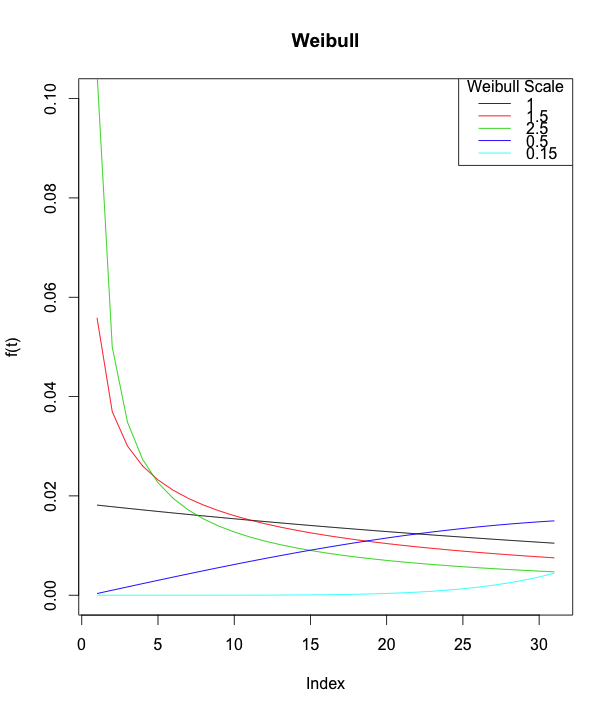
\includegraphics{/mnt/c/Users/ozd504/Documents/Github/DEM7223/images/weibull.png}

\begin{itemize}
\tightlist
\item
  Log-normal - another 2 parameter distribution, yes, the log of the
  Normal distribution. Strictly positive. Hazard function is this
  monster:
\end{itemize}

\[h(t) = \frac{\frac{1}{t\sigma \sqrt{2\pi}}exp \left [ \frac{-1}{2\sigma^2} {ln(t)-\mu}^2 \right]} {1-\Phi \left \{ \frac{ln(t)- \mu}{\sigma} \right \}} \]
\textbf{Yikes!} This is a much more flexible model, because the hazard
can actually increase and decrease, which the Weibull cannot do.

\begin{itemize}
\tightlist
\item
  Log-logistic - another 2 parameter distribution, very flexible
\end{itemize}

\[h(t) = \frac{\lambda \frac{1}{\gamma} t [ \frac{1}{\gamma} -1 ] }
{\gamma  [ 1+(\lambda t)^{\frac{1}{\gamma}} ]}\]

\textbf{Yikes!} If \(\gamma\) \textless{} then the hazard rises, then
falls, if \(\gamma \geqslant 1\), the hazard is declining The parameter
\(\lambda\) is the location, and can be parameterized as the linear mean
function: \(\lambda = e^{-{X'\beta}}\)

\begin{itemize}
\tightlist
\item
  Gompertz - very famous demographic model for adult mortality, hazard
  function is:
\end{itemize}

\[h(t) = \lambda e^{\gamma t} \] Where \(\lambda = e^{X'\beta}\)

If \(\gamma\) \textless{} 1, then the hazard is monotone decreasing over
time, if \(\gamma\) \textgreater1, then the hazard is increasing over
time, and if \(\gamma\) = 1 then the hazard is flat, and we have the
exponential.

In general, more parameters allow for more flexibility to the shape of
any distribution, and hence more flexibility when it comes to fitting
the distribution to data.

But be aware that more complicated models are not always better than
simple ones, and you should compare the fit of the model versus its
complexity

Parsimony is the backbone of science!

\hypertarget{more-on-the-exponential-model}{%
\subsubsection{More on the exponential
model}\label{more-on-the-exponential-model}}

\hypertarget{aft-form}{%
\subsubsection{AFT form}\label{aft-form}}

Since the exponential distribution is solely determined by the
parameter, λ, and λ\textgreater0, we need a model to accommodate this.
The exponential model can be specified two ways The accelerated failure
time model is:

\[log(T_i) = x'\beta + z_i\] Where the β's are regression parameters
relating covariate values (the x's) to the duration time

\hypertarget{ph-form}{%
\paragraph{PH form}\label{ph-form}}

If we treat the hazard rate, \(\lambda\), as a function of the
covariates and the \(\beta\)'s, we can write \(\lambda\) as

\[\lambda_i=exp^{(- x'β)}\] So the hazard rate, is given by the
covariates x

\hypertarget{more-on-proportional-hazards}{%
\subsubsection{More on proportional
hazards}\label{more-on-proportional-hazards}}

An important aspect of the exponential model is called the
\emph{proportional hazards interpretation} If x is either 1 or 0, and
the first term in the \(\beta\)'s is a constant (the intercept term), we
can write our hazard model as:

\[\frac{h_i(t|x=1)}{h_i(t|x=0)}= \frac{exp(-\beta_0 + \beta_1 * 1)}{exp(-\beta_0 + \beta_1 * 0)} = exp^{(\beta_1)}\]

So \(\beta\) is a constant, called the \emph{baseline hazard}

Changes to this baseline hazard happen through the effect of
\(\beta_1\), or the covariate effects, we can consider the relative
change in the hazard for someone with x =1, verses someone with x = 0

This is known as the \emph{proportional hazards property}

Since the hazard rate in the Exponential model is invariant with respect
to time, it represents a very simplistic model and one that often does
not occur in the real world

\hypertarget{be-careful-with-interpretations}{%
\subsubsection{Be careful with
interpretations!}\label{be-careful-with-interpretations}}

For Accelerated failure time model Y=log (duration), so if
\(exp(\beta_1) > 1\), you have an increase in time (implies a decrease
in risk), if \(exp(\beta_1) < 1\) you have a decrease in time (and an
implied increase in risk)

For Proportional Hazards models

Y=hazard(time), so if \(exp(\beta_1) > 1\), you have an increase in
hazard (and a decrease in duration), if \(exp(\beta_1) < 1\) you have a
decrease in hazard (and an increase in duration)

\hypertarget{data-example}{%
\subsection{Data example}\label{data-example}}

This example will illustrate how to fit parametric hazard models to
continuous duration data (i.e.~person-level data). In this example, I
use the \emph{time between the first and second birth} for women in the
data as the \emph{outcome variable}.

The data for this example come from the DHS Model data file
\href{https://t.co/tM8LfJhomf}{Demographic and Health Survey for 2012}
individual recode file. This file contains information for all women
sampled in the survey between the ages of 15 and 49.

This is an important data file, because for each woman, it gives
information on all of her births, arrayed in columns.

\begin{Shaded}
\begin{Highlighting}[]
\CommentTok{#Load required libraries}
\KeywordTok{library}\NormalTok{(haven)}
\KeywordTok{library}\NormalTok{(survival)}
\KeywordTok{library}\NormalTok{(car)}
\end{Highlighting}
\end{Shaded}

\begin{verbatim}
## Loading required package: carData
\end{verbatim}

\begin{Shaded}
\begin{Highlighting}[]
\KeywordTok{library}\NormalTok{(survey)}
\end{Highlighting}
\end{Shaded}

\begin{verbatim}
## Loading required package: grid
\end{verbatim}

\begin{verbatim}
## Loading required package: Matrix
\end{verbatim}

\begin{verbatim}
## 
## Attaching package: 'survey'
\end{verbatim}

\begin{verbatim}
## The following object is masked from 'package:graphics':
## 
##     dotchart
\end{verbatim}

\begin{Shaded}
\begin{Highlighting}[]
\KeywordTok{library}\NormalTok{(muhaz)}
\KeywordTok{library}\NormalTok{(eha)}

\CommentTok{#load the data}
\NormalTok{model.dat<-}\KeywordTok{read_dta}\NormalTok{(}\StringTok{"https://github.com/coreysparks/data/blob/master/ZZIR62FL.DTA?raw=true"}\NormalTok{)}
\NormalTok{model.dat<-}\KeywordTok{zap_labels}\NormalTok{(model.dat)}
\end{Highlighting}
\end{Shaded}

In the DHS individual recode file, information on every live birth is
collected using a retrospective birth history survey mechanism.

Since our outcome is time between first and second birth, we must select
as our risk set, only women who have had a first birth.

The \texttt{bidx} variable indexes the birth history and if
\texttt{bidx\_01} is not missing, then the woman should be at risk of
having a second birth (i.e.~she has had a first birth,
i.e.~\texttt{bidx\_01==1}).

I also select only non-twin births (\texttt{b0\ ==\ 0}).

The DHS provides the dates of when each child was born in Century Month
Codes.

To get the interval for women who \emph{actually had} a second birth,
that is the difference between the CMC for the first birth
\texttt{b3\_01} and the second birth \texttt{b3\_02}, but for women who
had not had a second birth by the time of the interview, the censored
time between births is the difference between \texttt{b3\_01} and
\texttt{v008}, the date of the interview.

We have 6161 women who are at risk of a second birth.

\begin{Shaded}
\begin{Highlighting}[]
\KeywordTok{table}\NormalTok{(}\KeywordTok{is.na}\NormalTok{(model.dat}\OperatorTok{$}\NormalTok{bidx_}\DecValTok{01}\NormalTok{))}
\end{Highlighting}
\end{Shaded}

\begin{verbatim}
## 
## FALSE  TRUE 
##  6161  2187
\end{verbatim}

\begin{Shaded}
\begin{Highlighting}[]
\CommentTok{#now we extract those women}
\NormalTok{sub<-}\KeywordTok{subset}\NormalTok{(model.dat, model.dat}\OperatorTok{$}\NormalTok{bidx_}\DecValTok{01}\OperatorTok{==}\DecValTok{1}\OperatorTok{&}\NormalTok{model.dat}\OperatorTok{$}\NormalTok{b0_}\DecValTok{01}\OperatorTok{==}\DecValTok{0}\NormalTok{)}

\CommentTok{#Here I keep only a few of the variables for the dates, and some characteristics of the women, and details of the survey}
\NormalTok{sub2<-}\KeywordTok{data.frame}\NormalTok{(}\DataTypeTok{CASEID=}\NormalTok{sub}\OperatorTok{$}\NormalTok{caseid, }
                 \DataTypeTok{int.cmc=}\NormalTok{sub}\OperatorTok{$}\NormalTok{v008,}
                 \DataTypeTok{fbir.cmc=}\NormalTok{sub}\OperatorTok{$}\NormalTok{b3_}\DecValTok{01}\NormalTok{,}
                 \DataTypeTok{sbir.cmc=}\NormalTok{sub}\OperatorTok{$}\NormalTok{b3_}\DecValTok{02}\NormalTok{,}
                 \DataTypeTok{marr.cmc=}\NormalTok{sub}\OperatorTok{$}\NormalTok{v509,}
                 \DataTypeTok{rural=}\NormalTok{sub}\OperatorTok{$}\NormalTok{v025,}
                 \DataTypeTok{educ=}\NormalTok{sub}\OperatorTok{$}\NormalTok{v106,}
                 \DataTypeTok{age=}\NormalTok{sub}\OperatorTok{$}\NormalTok{v012,}
                 \DataTypeTok{partneredu=}\NormalTok{sub}\OperatorTok{$}\NormalTok{v701,}
                 \DataTypeTok{partnerage=}\NormalTok{sub}\OperatorTok{$}\NormalTok{v730,}
                 \DataTypeTok{weight=}\NormalTok{sub}\OperatorTok{$}\NormalTok{v005}\OperatorTok{/}\DecValTok{1000000}\NormalTok{,}
                 \DataTypeTok{psu=}\NormalTok{sub}\OperatorTok{$}\NormalTok{v021, }\DataTypeTok{strata=}\NormalTok{sub}\OperatorTok{$}\NormalTok{v022)}

\NormalTok{sub2}\OperatorTok{$}\NormalTok{agefb =}\StringTok{ }\NormalTok{(sub2}\OperatorTok{$}\NormalTok{age }\OperatorTok{-}\StringTok{ }\NormalTok{(sub2}\OperatorTok{$}\NormalTok{int.cmc }\OperatorTok{-}\StringTok{ }\NormalTok{sub2}\OperatorTok{$}\NormalTok{fbir.cmc)}\OperatorTok{/}\DecValTok{12}\NormalTok{)}
\end{Highlighting}
\end{Shaded}

Now I need to calculate the birth intervals, both observed and censored,
and the event indicator (i.e.~did the women \emph{have} the second
birth?)

\begin{Shaded}
\begin{Highlighting}[]
\NormalTok{sub2}\OperatorTok{$}\NormalTok{secbi<-}\KeywordTok{ifelse}\NormalTok{(}\KeywordTok{is.na}\NormalTok{(sub2}\OperatorTok{$}\NormalTok{sbir.cmc)}\OperatorTok{==}\NormalTok{T,}
\NormalTok{                   ((sub2}\OperatorTok{$}\NormalTok{int.cmc))}\OperatorTok{-}\NormalTok{((sub2}\OperatorTok{$}\NormalTok{fbir.cmc)), }
\NormalTok{                   (sub2}\OperatorTok{$}\NormalTok{fbir.cmc}\OperatorTok{-}\NormalTok{sub2}\OperatorTok{$}\NormalTok{sbir.cmc))}

\NormalTok{sub2}\OperatorTok{$}\NormalTok{b2event<-}\KeywordTok{ifelse}\NormalTok{(}\KeywordTok{is.na}\NormalTok{(sub2}\OperatorTok{$}\NormalTok{sbir.cmc)}\OperatorTok{==}\NormalTok{T,}\DecValTok{0}\NormalTok{,}\DecValTok{1}\NormalTok{) }
\NormalTok{fit<-}\KeywordTok{survfit}\NormalTok{(}\KeywordTok{Surv}\NormalTok{(secbi, b2event)}\OperatorTok{~}\DecValTok{1}\NormalTok{, sub2)}
\NormalTok{fit}
\end{Highlighting}
\end{Shaded}

\begin{verbatim}
## Call: survfit(formula = Surv(secbi, b2event) ~ 1, data = sub2)
## 
##       n  events  median 0.95LCL 0.95UCL 
##    6026    4789      39      38      40
\end{verbatim}

\begin{Shaded}
\begin{Highlighting}[]
\KeywordTok{plot}\NormalTok{(fit, }\DataTypeTok{conf.int=}\NormalTok{T, }\DataTypeTok{ylab=}\StringTok{"S(t)"}\NormalTok{, }\DataTypeTok{xlab=}\StringTok{"Months"}\NormalTok{)}
\KeywordTok{title}\NormalTok{(}\DataTypeTok{main=}\StringTok{"Survival Function for Second Birth Interval, DHS Model Data"}\NormalTok{)}
\end{Highlighting}
\end{Shaded}

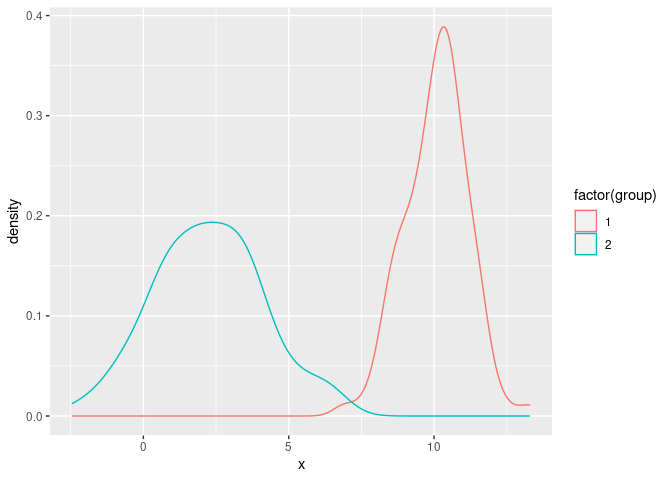
\includegraphics{EX3_Parametric_Hazard_Models_files/figure-latex/unnamed-chunk-3-1.pdf}

\hypertarget{estimating-parametric-hazard-models}{%
\subsubsection{Estimating Parametric Hazard
Models}\label{estimating-parametric-hazard-models}}

While parametric models are not so common in demographic research,
fundamental understanding of what they are and how they are constructed
is of importance.

Some outcomes lend themselves very readily to the parametric approach,
but as many demographic duration times are non-unique (tied), the
parametric models are not statistically efficient for estimating the
survival/hazard functions, as they assume the survival times are
continuous random variables.

In this section, we first estimate the empirical hazard function and
then fit a variety of parametric models to it (Exponential, Weibull,
Log-normal and Piecewise exponential). Ideally, a parametric model's
hazard function should approximate the observed empirical hazard
function, \emph{if the model fits the data}.

\begin{Shaded}
\begin{Highlighting}[]
\CommentTok{#since these functions don't work with durations of 0, we add a very small amount to the intervals}
\NormalTok{fit.haz.km<-}\KeywordTok{kphaz.fit}\NormalTok{(sub2}\OperatorTok{$}\NormalTok{secbi[sub2}\OperatorTok{$}\NormalTok{secbi}\OperatorTok{>}\DecValTok{0}\NormalTok{],}
\NormalTok{                      sub2}\OperatorTok{$}\NormalTok{b2event[sub2}\OperatorTok{$}\NormalTok{secbi}\OperatorTok{>}\DecValTok{0}\NormalTok{] , }
                      \DataTypeTok{method =} \StringTok{"product-limit"}\NormalTok{)}

\CommentTok{#this is a version of the hazard that is smoothed using a kernel-density method}
\NormalTok{fit.haz.sm<-}\KeywordTok{muhaz}\NormalTok{(sub2}\OperatorTok{$}\NormalTok{secbi[sub2}\OperatorTok{$}\NormalTok{secbi}\OperatorTok{>}\DecValTok{0}\NormalTok{], sub2}\OperatorTok{$}\NormalTok{b2event[sub2}\OperatorTok{$}\NormalTok{secbi}\OperatorTok{>}\DecValTok{0}\NormalTok{] )}

\CommentTok{#Empirical hazard function (product-limit estimate) plot}
\KeywordTok{kphaz.plot}\NormalTok{(fit.haz.km,}\DataTypeTok{main=}\StringTok{"Plot of the hazard of having a second birth"}\NormalTok{)}
\CommentTok{#overlay the smoothed version}
\KeywordTok{lines}\NormalTok{(fit.haz.sm, }\DataTypeTok{col=}\DecValTok{2}\NormalTok{, }\DataTypeTok{lwd=}\DecValTok{3}\NormalTok{)}
\KeywordTok{legend}\NormalTok{(}\StringTok{"topleft"}\NormalTok{, }\DataTypeTok{legend =} \KeywordTok{c}\NormalTok{(}\StringTok{"KM hazard"}\NormalTok{, }\StringTok{"Smoothed Hazard"}\NormalTok{),}
       \DataTypeTok{col=}\KeywordTok{c}\NormalTok{(}\DecValTok{1}\NormalTok{,}\DecValTok{2}\NormalTok{), }\DataTypeTok{lty=}\KeywordTok{c}\NormalTok{(}\DecValTok{1}\NormalTok{,}\DecValTok{1}\NormalTok{))}
\end{Highlighting}
\end{Shaded}

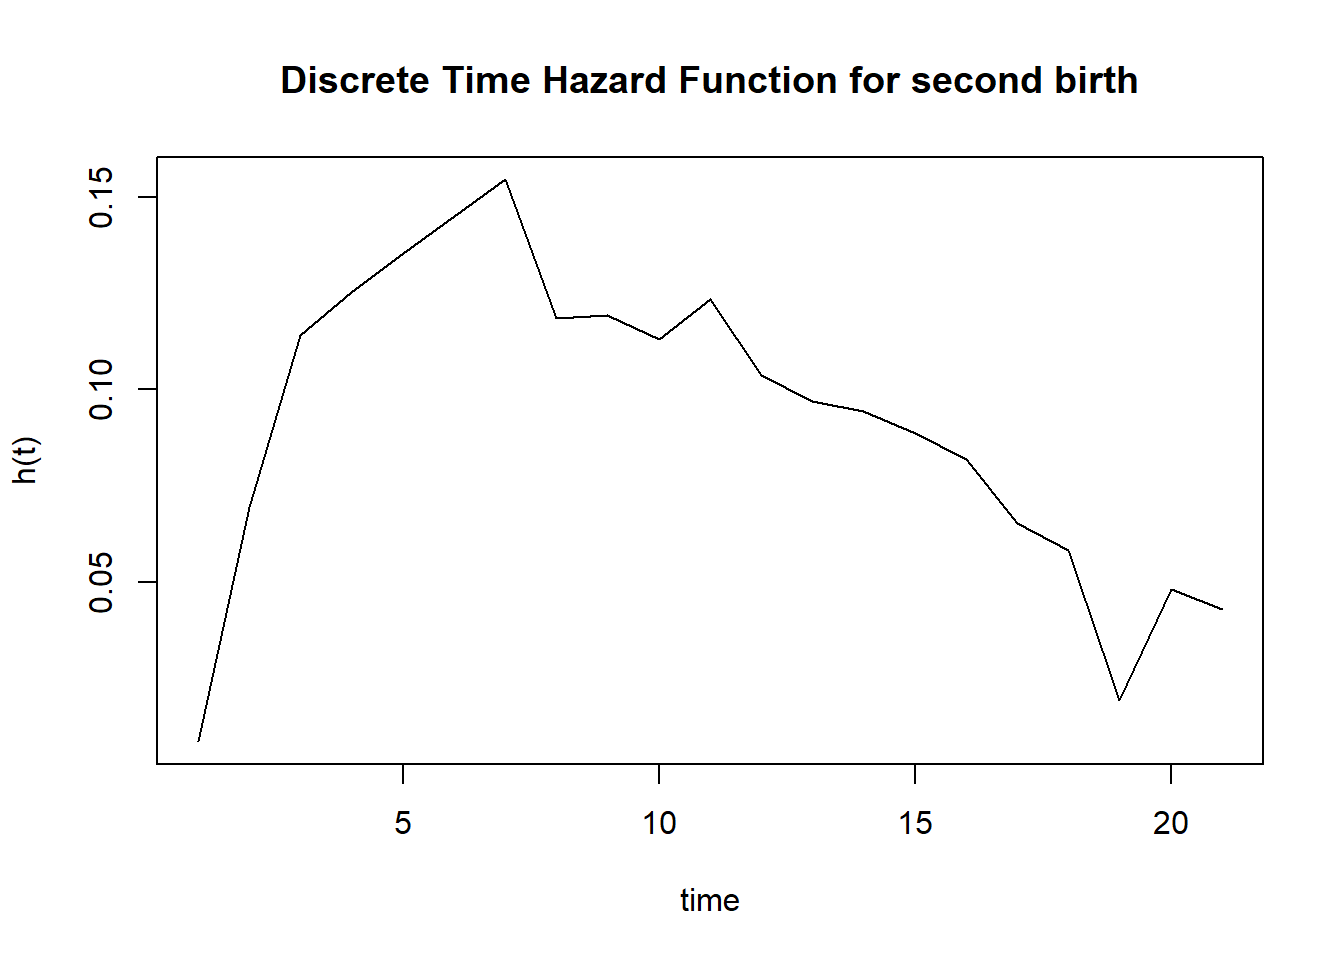
\includegraphics{EX3_Parametric_Hazard_Models_files/figure-latex/unnamed-chunk-4-1.pdf}

So now we see what the empirical hazard function looks like, in both the
observed and smoothed estimate of it.

\hypertarget{create-covariates}{%
\subsubsection{Create covariates}\label{create-covariates}}

Here, we create some predictor variables: Woman's education (secondary
+, vs \textless{} secondary), Woman's age\^{}2, Partner's education
(\textgreater{} secondary school)

\begin{Shaded}
\begin{Highlighting}[]
\NormalTok{sub2}\OperatorTok{$}\NormalTok{educ.high<-}\KeywordTok{ifelse}\NormalTok{(sub2}\OperatorTok{$}\NormalTok{educ }\OperatorTok\StringTok{ }\KeywordTok{c}\NormalTok{(}\DecValTok{2}\NormalTok{,}\DecValTok{3}\NormalTok{), }\DecValTok{1}\NormalTok{, }\DecValTok{0}\NormalTok{)}
\NormalTok{sub2}\OperatorTok{$}\NormalTok{age2<-(sub2}\OperatorTok{$}\NormalTok{agefb}\OperatorTok{/}\DecValTok{5}\NormalTok{)}\OperatorTok{^}\DecValTok{2}
\NormalTok{sub2}\OperatorTok{$}\NormalTok{partnerhiedu<-}\KeywordTok{ifelse}\NormalTok{(sub2}\OperatorTok{$}\NormalTok{partneredu}\OperatorTok{<}\DecValTok{3}\NormalTok{,}\DecValTok{0}\NormalTok{,}
                          \KeywordTok{ifelse}\NormalTok{(sub2}\OperatorTok{$}\NormalTok{partneredu}\OperatorTok\KeywordTok{c}\NormalTok{(}\DecValTok{8}\NormalTok{,}\DecValTok{9}\NormalTok{),}\OtherTok{NA}\NormalTok{,}\DecValTok{1}\NormalTok{ ))}

\KeywordTok{options}\NormalTok{(}\DataTypeTok{survey.lonely.psu =} \StringTok{"adjust"}\NormalTok{)}
\NormalTok{des<-}\KeywordTok{svydesign}\NormalTok{(}\DataTypeTok{ids=}\OperatorTok{~}\NormalTok{psu, }\DataTypeTok{strata=}\OperatorTok{~}\NormalTok{strata,}
               \DataTypeTok{data=}\NormalTok{sub2[sub2}\OperatorTok{$}\NormalTok{secbi}\OperatorTok{>}\DecValTok{0}\NormalTok{,], }\DataTypeTok{weight=}\OperatorTok{~}\NormalTok{weight )}

\NormalTok{rep.des<-}\KeywordTok{as.svrepdesign}\NormalTok{(des, }\DataTypeTok{type=}\StringTok{"bootstrap"}\NormalTok{ )}
\end{Highlighting}
\end{Shaded}

\hypertarget{fit-the-models}{%
\section{Fit the models}\label{fit-the-models}}

Now we fit the models.

I use the \texttt{eha}
\href{http://cran.r-project.org/web/packages/eha/index.html}{package} to
do this, since it fits parametric proportional hazard models, not
accelerated failure time models.

I prefer the interpretation of regression models on the hazard scale
vs.~the survival time scale. EHA is not the only package that will fit
parametric survival models, be sure you \emph{read the documentation for
the procedure you use!!} Different functions fit different
parameterizations of the distributions. For example, the
\texttt{survreg()} function in the \texttt{survival} library fits
accelerated failure time models only.

\hypertarget{exponential-model}{%
\subsubsection{Exponential Model}\label{exponential-model}}

Often the exponential model isn't directly available in packages, so we
can fit a weibull model with a fixed shape parameter. This is 100\%
legal.

The exponential distribution has a constant hazard rate,
\(\lambda (t) = \lambda\). The survival function is
\(S(t) = \exp (-\lambda t)\)

To specify the model in terms of covariates, you can write the hazard as
a log-linear model : \(\text{log} \lambda = x`\beta\)

\begin{Shaded}
\begin{Highlighting}[]
\CommentTok{#exponential distribution for hazard, here we hard code it to be}
\CommentTok{#a weibull dist with shape ==1 }
\NormalTok{fit}\FloatTok{.1}\NormalTok{<-}\KeywordTok{phreg}\NormalTok{(}\KeywordTok{Surv}\NormalTok{(secbi, b2event)}\OperatorTok{~}\NormalTok{educ.high}\OperatorTok{+}\NormalTok{partnerhiedu}\OperatorTok{+}\KeywordTok{I}\NormalTok{(agefb}\OperatorTok{/}\DecValTok{5}\NormalTok{)}\OperatorTok{+}\NormalTok{age2,}
             \DataTypeTok{data=}\NormalTok{sub2[sub2}\OperatorTok{$}\NormalTok{secbi}\OperatorTok{>}\DecValTok{0}\NormalTok{,], }\DataTypeTok{dist=}\StringTok{"weibull"}\NormalTok{, }\DataTypeTok{shape =} \DecValTok{1}\NormalTok{)}
\KeywordTok{summary}\NormalTok{(fit}\FloatTok{.1}\NormalTok{)}
\end{Highlighting}
\end{Shaded}

\begin{verbatim}
## Call:
## phreg(formula = Surv(secbi, b2event) ~ educ.high + partnerhiedu + 
##     I(agefb/5) + age2, data = sub2[sub2$secbi > 0, ], dist = "weibull", 
##     shape = 1)
## 
## Covariate          W.mean      Coef Exp(Coef)  se(Coef)    Wald p
## educ.high           0.167    -0.280     0.756     0.048     0.000 
## partnerhiedu        0.071    -0.180     0.835     0.069     0.009 
## I(agefb/5)          5.744     1.130     3.095     0.084     0.000 
## age2               35.186    -0.090     0.914     0.007     0.000 
## 
## log(scale)                    7.254               0.244     0.000 
## 
##  Shape is fixed at  1 
## 
## Events                    4527 
## Total time at risk        237141 
## Max. log. likelihood      -22296 
## LR test statistic         303.75 
## Degrees of freedom        4 
## Overall p-value           0
\end{verbatim}

\begin{Shaded}
\begin{Highlighting}[]
\KeywordTok{plot}\NormalTok{(fit}\FloatTok{.1}\NormalTok{)}
\end{Highlighting}
\end{Shaded}

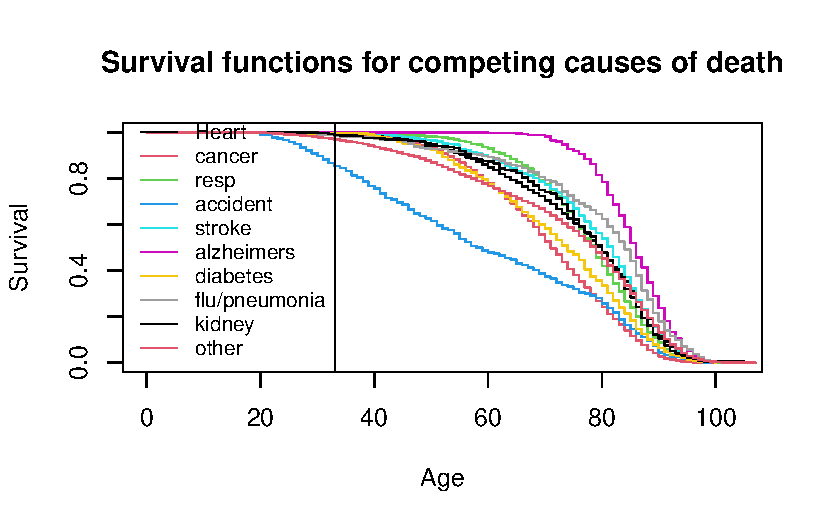
\includegraphics{EX3_Parametric_Hazard_Models_files/figure-latex/unnamed-chunk-6-1.pdf}

Which shows us what the constant hazard model looks like, it assumed the
hazard is constant with respect to time, which after seeing the plots
above, we know is false. We see the effects of both woman's and
partner's education are negative, which makes sense. Women with more
education, and who have partners with more education lower risks of
having a second birth. We also see the age effect is significant,
meaning older women in this sample are more likely to have a second
birth but the hazard doesn't go up forever, as the curvilinear term
shows a negative slope.

\#\#\#Interpreting the model coefficients To interpret the effects
specifically, you can use the \texttt{Exp(Coef)} column. So, for example
for women who have secondary or higher education, their hazard of having
a second child is 24.436 lower than a woman with less than a secondary
education. To get that number I do :
\(100* 1 - \exp(\beta_{\text{educ.high }})\)

Likewise, for the effect of age, we can compare the hazards for a women
who is age 35 to a woman who is age 20. To do this comparison for a
continuous covariate, you have to form the ratio of the hazards at two
different plausible values. For this comparison, we see that women who
are age 35 are 1.512 times more likely to have a second birth than women
who are 20. To get this, I find:

\(\text{Hazard Ratio} = \frac{\exp \left( \beta_{\text{I(age/5)}} * 7 + \beta_{\text{age2}}*7 \right )}{\exp \left( \beta_{\text{I(age/5)}} * 4 + \beta_{\text{age2}}*4 \right )}\)

I choose 7 because \texttt{7\ *\ 5} = 35, and 4 because \texttt{4*5} =
20. Remember, I divided Age by 5 when I created my variables.

\hypertarget{aft-model-specification}{%
\subsubsection{AFT model specification}\label{aft-model-specification}}

If you wanted to do the AFT model, you can either \texttt{aftreg()} in
the \texttt{eha} package or \texttt{survreg()} in the \texttt{survival}
package. Generally AFT models are written as:

\(\text{log} T = -x ` \beta + \sigma W\) Where \emph{W} is an error
(residual) term, which is assumed to follow some distribution.

\begin{Shaded}
\begin{Highlighting}[]
\NormalTok{fit.}\FloatTok{1.}\NormalTok{aft<-}\KeywordTok{survreg}\NormalTok{(}\KeywordTok{Surv}\NormalTok{(secbi, b2event)}\OperatorTok{~}\NormalTok{educ.high}\OperatorTok{+}\NormalTok{partnerhiedu}\OperatorTok{+}\KeywordTok{I}\NormalTok{(age}\OperatorTok{/}\DecValTok{5}\NormalTok{)}\OperatorTok{+}\NormalTok{age2 }\OperatorTok{+}\StringTok{ }\NormalTok{age2,}
                   \DataTypeTok{data=}\NormalTok{sub2[sub2}\OperatorTok{$}\NormalTok{secbi}\OperatorTok{>}\DecValTok{0}\NormalTok{,],}\DataTypeTok{dist =} \StringTok{"exponential"}\NormalTok{)}

\KeywordTok{summary}\NormalTok{(fit.}\FloatTok{1.}\NormalTok{aft)}
\end{Highlighting}
\end{Shaded}

\begin{verbatim}
## 
## Call:
## survreg(formula = Surv(secbi, b2event) ~ educ.high + partnerhiedu + 
##     I(age/5) + age2 + age2, data = sub2[sub2$secbi > 0, ], dist = "exponential")
##                 Value Std. Error     z       p
## (Intercept)   3.45845    0.07168 48.25 < 2e-16
## educ.high     0.29630    0.04791  6.18 6.2e-10
## partnerhiedu  0.12346    0.06859  1.80   0.072
## I(age/5)      0.13581    0.01511  8.99 < 2e-16
## age2         -0.01326    0.00138 -9.62 < 2e-16
## 
## Scale fixed at 1 
## 
## Exponential distribution
## Loglik(model)= -22354.2   Loglik(intercept only)= -22447.6
##  Chisq= 186.77 on 4 degrees of freedom, p= 2.6e-39 
## Number of Newton-Raphson Iterations: 4 
## n=5279 (728 observations deleted due to missingness)
\end{verbatim}

Which shows, compared to the PH model, that the coefficients are all
backwards. That's because if a predictor lowers the hazard, then, by
default it extends survival.

\hypertarget{lower-risk-longer-survival-times}{%
\subsubsection{Lower risk == longer survival
times!}\label{lower-risk-longer-survival-times}}

\hypertarget{weibull-model}{%
\subsubsection{Weibull Model}\label{weibull-model}}

The Weibull model is more flexible than the Exponential, because it's
distribution function has two parameters, scale and shape.

The Weibull distribution has hazard rate,
\(\lambda(t)=\lambda^p p t^{p-1}\). Where \(\lambda\) is the scale and
\emph{p} is the shape. The survival function is
\(S(t) = exp ( -(\lambda t)^p)\)

\begin{Shaded}
\begin{Highlighting}[]
\CommentTok{#weibull distribution for hazard}
\NormalTok{fit}\FloatTok{.2}\NormalTok{<-}\KeywordTok{phreg}\NormalTok{(}\KeywordTok{Surv}\NormalTok{(secbi, b2event)}\OperatorTok{~}\NormalTok{educ.high}\OperatorTok{+}\NormalTok{partnerhiedu}\OperatorTok{+}\KeywordTok{I}\NormalTok{(age}\OperatorTok{/}\DecValTok{5}\NormalTok{)}\OperatorTok{+}\NormalTok{age2,}
             \DataTypeTok{data=}\NormalTok{sub2[sub2}\OperatorTok{$}\NormalTok{secbi}\OperatorTok{>}\DecValTok{0}\NormalTok{,], }\DataTypeTok{dist=}\StringTok{"weibull"}\NormalTok{)}
\KeywordTok{summary}\NormalTok{(fit}\FloatTok{.2}\NormalTok{)}
\end{Highlighting}
\end{Shaded}

\begin{verbatim}
## Call:
## phreg(formula = Surv(secbi, b2event) ~ educ.high + partnerhiedu + 
##     I(age/5) + age2, data = sub2[sub2$secbi > 0, ], dist = "weibull")
## 
## Covariate          W.mean      Coef Exp(Coef)  se(Coef)    Wald p
## educ.high           0.167    -0.369     0.691     0.048     0.000 
## partnerhiedu        0.071    -0.229     0.796     0.068     0.001 
## I(age/5)            6.859    -0.340     0.712     0.016     0.000 
## age2               35.186     0.024     1.024     0.001     0.000 
## 
## log(scale)                    3.133               0.043     0.000 
## log(shape)                    0.525               0.011     0.000 
## 
## Events                    4527 
## Total time at risk        237141 
## Max. log. likelihood      -21461 
## LR test statistic         684.43 
## Degrees of freedom        4 
## Overall p-value           0
\end{verbatim}

\begin{Shaded}
\begin{Highlighting}[]
\KeywordTok{plot}\NormalTok{(fit}\FloatTok{.2}\NormalTok{)}
\end{Highlighting}
\end{Shaded}

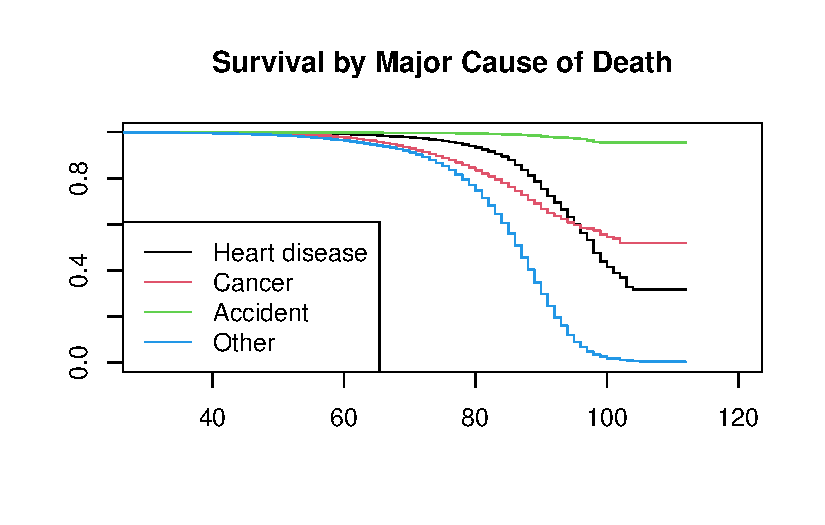
\includegraphics{EX3_Parametric_Hazard_Models_files/figure-latex/unnamed-chunk-8-1.pdf}

\begin{Shaded}
\begin{Highlighting}[]
\KeywordTok{plot}\NormalTok{(fit}\FloatTok{.2}\NormalTok{, }\DataTypeTok{fn=}\StringTok{"haz"}\NormalTok{)}
\KeywordTok{lines}\NormalTok{(fit.haz.sm, }\DataTypeTok{col=}\DecValTok{2}\NormalTok{)}
\end{Highlighting}
\end{Shaded}

\includegraphics{EX3_Parametric_Hazard_Models_files/figure-latex/unnamed-chunk-8-2.pdf}

Here, we see a more realistic situation, where the hazard function
changes over time (Weibull allows this), but compared to the empirical
hazard, the model is a very poor fit, as empirically, the hazard goes
up, but then goes down. The Weibull hazard just goes up, as the model
does not allow the hazard to change direction, only rate of increase
(i.e.~it can increase at a slower or faster rate, but not change
direction). We see the Age effects begin to go away, because the
baseline hazard is accounting for the age effects on fertility.

\#\#Note on exponential and Weibull models AFT vs PH parameterization
and, as a nice trick for the exponential and weibull models, you can
rescale the AFT beta's to PH model betas (see
\href{http://www.statisticsmentor.com/2012/12/25/r-relationship-between-accelerated-failure-model-and-the-proportional-hazard-model-for-weibull/}{here})

\begin{Shaded}
\begin{Highlighting}[]
\CommentTok{#re-scaled beta's}
\NormalTok{(betaHat <-}\StringTok{ }\OperatorTok{-}\KeywordTok{coef}\NormalTok{(fit.}\FloatTok{1.}\NormalTok{aft) }\OperatorTok{/}\StringTok{ }\NormalTok{fit.}\FloatTok{1.}\NormalTok{aft}\OperatorTok{$}\NormalTok{scale)}
\end{Highlighting}
\end{Shaded}

\begin{verbatim}
##  (Intercept)    educ.high partnerhiedu     I(age/5)         age2 
##  -3.45844846  -0.29630384  -0.12346198  -0.13580668   0.01326201
\end{verbatim}

\begin{Shaded}
\begin{Highlighting}[]
\CommentTok{#beta's from the PH model}
\KeywordTok{coef}\NormalTok{(fit}\FloatTok{.1}\NormalTok{)}
\end{Highlighting}
\end{Shaded}

\begin{verbatim}
##    educ.high partnerhiedu   I(agefb/5)         age2   log(scale) 
##  -0.28019154  -0.17987145   1.12983459  -0.09019032   7.25416728
\end{verbatim}

So for these two models, you can go back and forth.

\hypertarget{log-normal-model}{%
\subsubsection{Log-Normal Model}\label{log-normal-model}}

The Log-normal distribution is more flexible and allows the hazard to
change direction.

The Log-normal distribution has hazard rate,
\(h(t) = \frac{\phi \left (\frac{log t}{\sigma} \right ) }{\left [ 1 - \Phi \left ( \frac{log t}{\sigma} \right ) \right ] \sigma t}\)

. Where \(\sigma\) is the shape.

The survival function is
\(S(t) = 1 - \Phi \left ( \frac{log t - \mu}{\sigma} \right )\)

\begin{Shaded}
\begin{Highlighting}[]
\CommentTok{#log-normal distribution for hazard}
\NormalTok{fit}\FloatTok{.3}\NormalTok{<-}\KeywordTok{phreg}\NormalTok{(}\KeywordTok{Surv}\NormalTok{(secbi, b2event)}\OperatorTok{~}\NormalTok{educ.high}\OperatorTok{+}\NormalTok{partnerhiedu}\OperatorTok{+}\KeywordTok{I}\NormalTok{(age}\OperatorTok{/}\DecValTok{5}\NormalTok{)}\OperatorTok{+}\NormalTok{age2,}
             \DataTypeTok{data=}\NormalTok{sub2[sub2}\OperatorTok{$}\NormalTok{secbi}\OperatorTok{>}\DecValTok{0}\NormalTok{,], }\DataTypeTok{dist=}\StringTok{"lognormal"}\NormalTok{, }\DataTypeTok{center=}\NormalTok{T)}
\KeywordTok{summary}\NormalTok{(fit}\FloatTok{.3}\NormalTok{)}
\end{Highlighting}
\end{Shaded}

\begin{verbatim}
## Call:
## phreg(formula = Surv(secbi, b2event) ~ educ.high + partnerhiedu + 
##     I(age/5) + age2, data = sub2[sub2$secbi > 0, ], dist = "lognormal", 
##     center = T)
## 
## Covariate          W.mean      Coef Exp(Coef)  se(Coef)    Wald p
## (Intercept)                  -1.002               0.170     0.000 
## educ.high           0.167    -0.350     0.705     0.048     0.000 
## partnerhiedu        0.071    -0.196     0.822     0.068     0.004 
## I(age/5)            6.859    -0.208     0.813     0.016     0.000 
## age2               35.186     0.014     1.014     0.001     0.000 
## 
## log(scale)                    2.997               0.037     0.000 
## log(shape)                    1.267               0.055     0.000 
## 
## Events                    4527 
## Total time at risk        237141 
## Max. log. likelihood      -20596 
## LR test statistic         303.40 
## Degrees of freedom        4 
## Overall p-value           0
\end{verbatim}

\begin{Shaded}
\begin{Highlighting}[]
\KeywordTok{plot}\NormalTok{(fit}\FloatTok{.3}\NormalTok{)}
\end{Highlighting}
\end{Shaded}

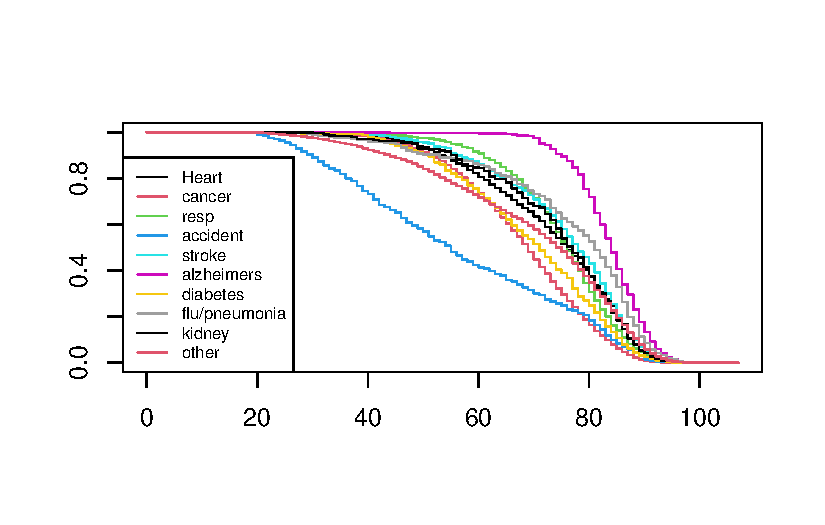
\includegraphics{EX3_Parametric_Hazard_Models_files/figure-latex/unnamed-chunk-10-1.pdf}

\begin{Shaded}
\begin{Highlighting}[]
\CommentTok{#plot the hazard from the log normal vs the empirical hazard}
\KeywordTok{plot}\NormalTok{(fit}\FloatTok{.3}\NormalTok{, }\DataTypeTok{fn=}\StringTok{"haz"}\NormalTok{)}
\KeywordTok{lines}\NormalTok{(fit.haz.sm, }\DataTypeTok{col=}\DecValTok{2}\NormalTok{)}
\end{Highlighting}
\end{Shaded}

\includegraphics{EX3_Parametric_Hazard_Models_files/figure-latex/unnamed-chunk-10-2.pdf}

We now see the age effect completely gone from the model.

So, the log-normal model fits the empirical hazard pretty well up to
\textasciitilde150 months, where the empirical rate drops off faster.
The \texttt{eha} package allows one other parametric distribution, the
log-logistic, so we will consider that one too:

\textbf{Log-logistic Model}

\begin{Shaded}
\begin{Highlighting}[]
\CommentTok{#log-normal distribution for hazard}
\NormalTok{fit}\FloatTok{.4}\NormalTok{<-}\KeywordTok{phreg}\NormalTok{(}\KeywordTok{Surv}\NormalTok{(secbi, b2event)}\OperatorTok{~}\NormalTok{educ.high}\OperatorTok{+}\NormalTok{partnerhiedu}\OperatorTok{+}\KeywordTok{I}\NormalTok{(age}\OperatorTok{/}\DecValTok{5}\NormalTok{)}\OperatorTok{+}\NormalTok{age2,}
             \DataTypeTok{data=}\NormalTok{sub2[sub2}\OperatorTok{$}\NormalTok{secbi}\OperatorTok{>}\DecValTok{0}\NormalTok{,], }\DataTypeTok{dist=}\StringTok{"loglogistic"}\NormalTok{, }\DataTypeTok{center=}\NormalTok{T)}
\KeywordTok{summary}\NormalTok{(fit}\FloatTok{.4}\NormalTok{)}
\end{Highlighting}
\end{Shaded}

\begin{verbatim}
## Call:
## phreg(formula = Surv(secbi, b2event) ~ educ.high + partnerhiedu + 
##     I(age/5) + age2, data = sub2[sub2$secbi > 0, ], dist = "loglogistic", 
##     center = T)
## 
## Covariate          W.mean      Coef Exp(Coef)  se(Coef)    Wald p
## (Intercept)                  -0.121               0.095     0.202 
## educ.high           0.167    -0.338     0.713     0.048     0.000 
## partnerhiedu        0.071    -0.185     0.831     0.068     0.007 
## I(age/5)            6.859    -0.154     0.857     0.016     0.000 
## age2               35.186     0.011     1.011     0.001     0.000 
## 
## log(scale)                    3.336               0.018     0.000 
## log(shape)                    1.534               0.028     0.000 
## 
## Events                    4527 
## Total time at risk        237141 
## Max. log. likelihood      -20534 
## LR test statistic         199.20 
## Degrees of freedom        4 
## Overall p-value           0
\end{verbatim}

\begin{Shaded}
\begin{Highlighting}[]
\KeywordTok{plot}\NormalTok{(fit}\FloatTok{.4}\NormalTok{)}
\end{Highlighting}
\end{Shaded}

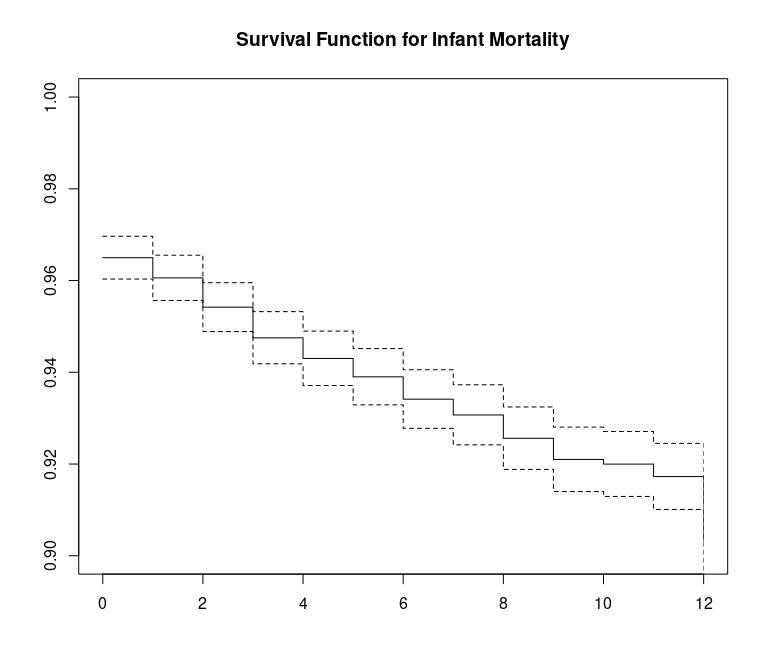
\includegraphics{EX3_Parametric_Hazard_Models_files/figure-latex/unnamed-chunk-11-1.pdf}

\begin{Shaded}
\begin{Highlighting}[]
\CommentTok{#plot the hazard from the log normal vs the empirical hazard}
\KeywordTok{plot}\NormalTok{(fit}\FloatTok{.4}\NormalTok{, }\DataTypeTok{fn=}\StringTok{"haz"}\NormalTok{)}
\KeywordTok{lines}\NormalTok{(fit.haz.sm, }\DataTypeTok{col=}\DecValTok{2}\NormalTok{)}
\end{Highlighting}
\end{Shaded}

\includegraphics{EX3_Parametric_Hazard_Models_files/figure-latex/unnamed-chunk-11-2.pdf}

Whose hazard function drops off faster than the log-normal.

We may want to compare the models to one another based off AIC values.
the \texttt{eha} package doesn't give this to you, so we must calculate
it:

\begin{Shaded}
\begin{Highlighting}[]
\NormalTok{AIC1<-}\OperatorTok{-}\DecValTok{2}\OperatorTok{*}\NormalTok{fit}\FloatTok{.1}\OperatorTok{$}\NormalTok{loglik[}\DecValTok{2}\NormalTok{]}\OperatorTok{+}\DecValTok{2}\OperatorTok{*}\KeywordTok{length}\NormalTok{(fit}\FloatTok{.1}\OperatorTok{$}\NormalTok{coefficients); AIC1}
\end{Highlighting}
\end{Shaded}

\begin{verbatim}
## [1] 44601.37
\end{verbatim}

\begin{Shaded}
\begin{Highlighting}[]
\NormalTok{AIC2<-}\OperatorTok{-}\DecValTok{2}\OperatorTok{*}\NormalTok{fit}\FloatTok{.2}\OperatorTok{$}\NormalTok{loglik[}\DecValTok{2}\NormalTok{]}\OperatorTok{+}\DecValTok{2}\OperatorTok{*}\KeywordTok{length}\NormalTok{(fit}\FloatTok{.2}\OperatorTok{$}\NormalTok{coefficients); AIC2}
\end{Highlighting}
\end{Shaded}

\begin{verbatim}
## [1] 42933.17
\end{verbatim}

\begin{Shaded}
\begin{Highlighting}[]
\NormalTok{AIC3<-}\OperatorTok{-}\DecValTok{2}\OperatorTok{*}\NormalTok{fit}\FloatTok{.3}\OperatorTok{$}\NormalTok{loglik[}\DecValTok{2}\NormalTok{]}\OperatorTok{+}\DecValTok{2}\OperatorTok{*}\KeywordTok{length}\NormalTok{(fit}\FloatTok{.3}\OperatorTok{$}\NormalTok{coefficients); AIC3}
\end{Highlighting}
\end{Shaded}

\begin{verbatim}
## [1] 41206.94
\end{verbatim}

\begin{Shaded}
\begin{Highlighting}[]
\NormalTok{AIC4<-}\OperatorTok{-}\DecValTok{2}\OperatorTok{*}\NormalTok{fit}\FloatTok{.4}\OperatorTok{$}\NormalTok{loglik[}\DecValTok{2}\NormalTok{]}\OperatorTok{+}\DecValTok{2}\OperatorTok{*}\KeywordTok{length}\NormalTok{(fit}\FloatTok{.4}\OperatorTok{$}\NormalTok{coefficients); AIC4}
\end{Highlighting}
\end{Shaded}

\begin{verbatim}
## [1] 41082
\end{verbatim}

And we see the log-logistic model best fits the data, based on the
minimum AIC criteria

\hypertarget{piecewise-constant-exponential-model}{%
\subsubsection{Piecewise constant exponential
model}\label{piecewise-constant-exponential-model}}

The final model we consider is the Piecewise constant exponential model.
This model breaks the data into pieces, where we may fit constant
hazards within these pieces.

For instance, given the observed hazard function above, we may break the
data into an early piece, say \textless{} 30 months, a high piece,30-80
months and maybe two low pieces (80-150 and \textgreater150), so to
mimic the form of the hazard function.

\begin{Shaded}
\begin{Highlighting}[]
\CommentTok{# here I must supply the times for the "pieces" where I expect the  hazard to be constant}
\NormalTok{fit}\FloatTok{.5}\NormalTok{<-}\KeywordTok{phreg}\NormalTok{(}\KeywordTok{Surv}\NormalTok{(secbi, b2event)}\OperatorTok{~}\NormalTok{educ.high}\OperatorTok{+}\NormalTok{partnerhiedu}\OperatorTok{+}\KeywordTok{I}\NormalTok{(age}\OperatorTok{/}\DecValTok{5}\NormalTok{)}\OperatorTok{+}\NormalTok{age2,}
             \DataTypeTok{data=}\NormalTok{sub2[sub2}\OperatorTok{$}\NormalTok{secbi}\OperatorTok{>}\DecValTok{0}\NormalTok{,], }\DataTypeTok{dist=}\StringTok{"pch"}\NormalTok{,}
             \DataTypeTok{cuts=}\KeywordTok{c}\NormalTok{(}\DecValTok{30}\NormalTok{, }\DecValTok{80}\NormalTok{, }\DecValTok{150}\NormalTok{,}\DecValTok{250}\NormalTok{))}
\KeywordTok{summary}\NormalTok{(fit}\FloatTok{.5}\NormalTok{)}
\end{Highlighting}
\end{Shaded}

\begin{verbatim}
## Call:
## phreg(formula = Surv(secbi, b2event) ~ educ.high + partnerhiedu + 
##     I(age/5) + age2, data = sub2[sub2$secbi > 0, ], dist = "pch", 
##     cuts = c(30, 80, 150, 250))
## 
## Covariate          W.mean      Coef Exp(Coef)  se(Coef)    Wald p
## educ.high           0.167    -0.345     0.708     0.048     0.000 
## partnerhiedu        0.071    -0.175     0.839     0.068     0.011 
## I(age/5)            6.859    -0.158     0.853     0.016     0.000 
## age2               35.186     0.012     1.012     0.001     0.000 
## 
## 
## Events                    4527 
## Total time at risk        237141 
## Max. log. likelihood      -21695 
## LR test statistic         201.04 
## Degrees of freedom        4 
## Overall p-value           0
\end{verbatim}

\begin{Shaded}
\begin{Highlighting}[]
\KeywordTok{plot}\NormalTok{(fit}\FloatTok{.5}\NormalTok{)}
\end{Highlighting}
\end{Shaded}

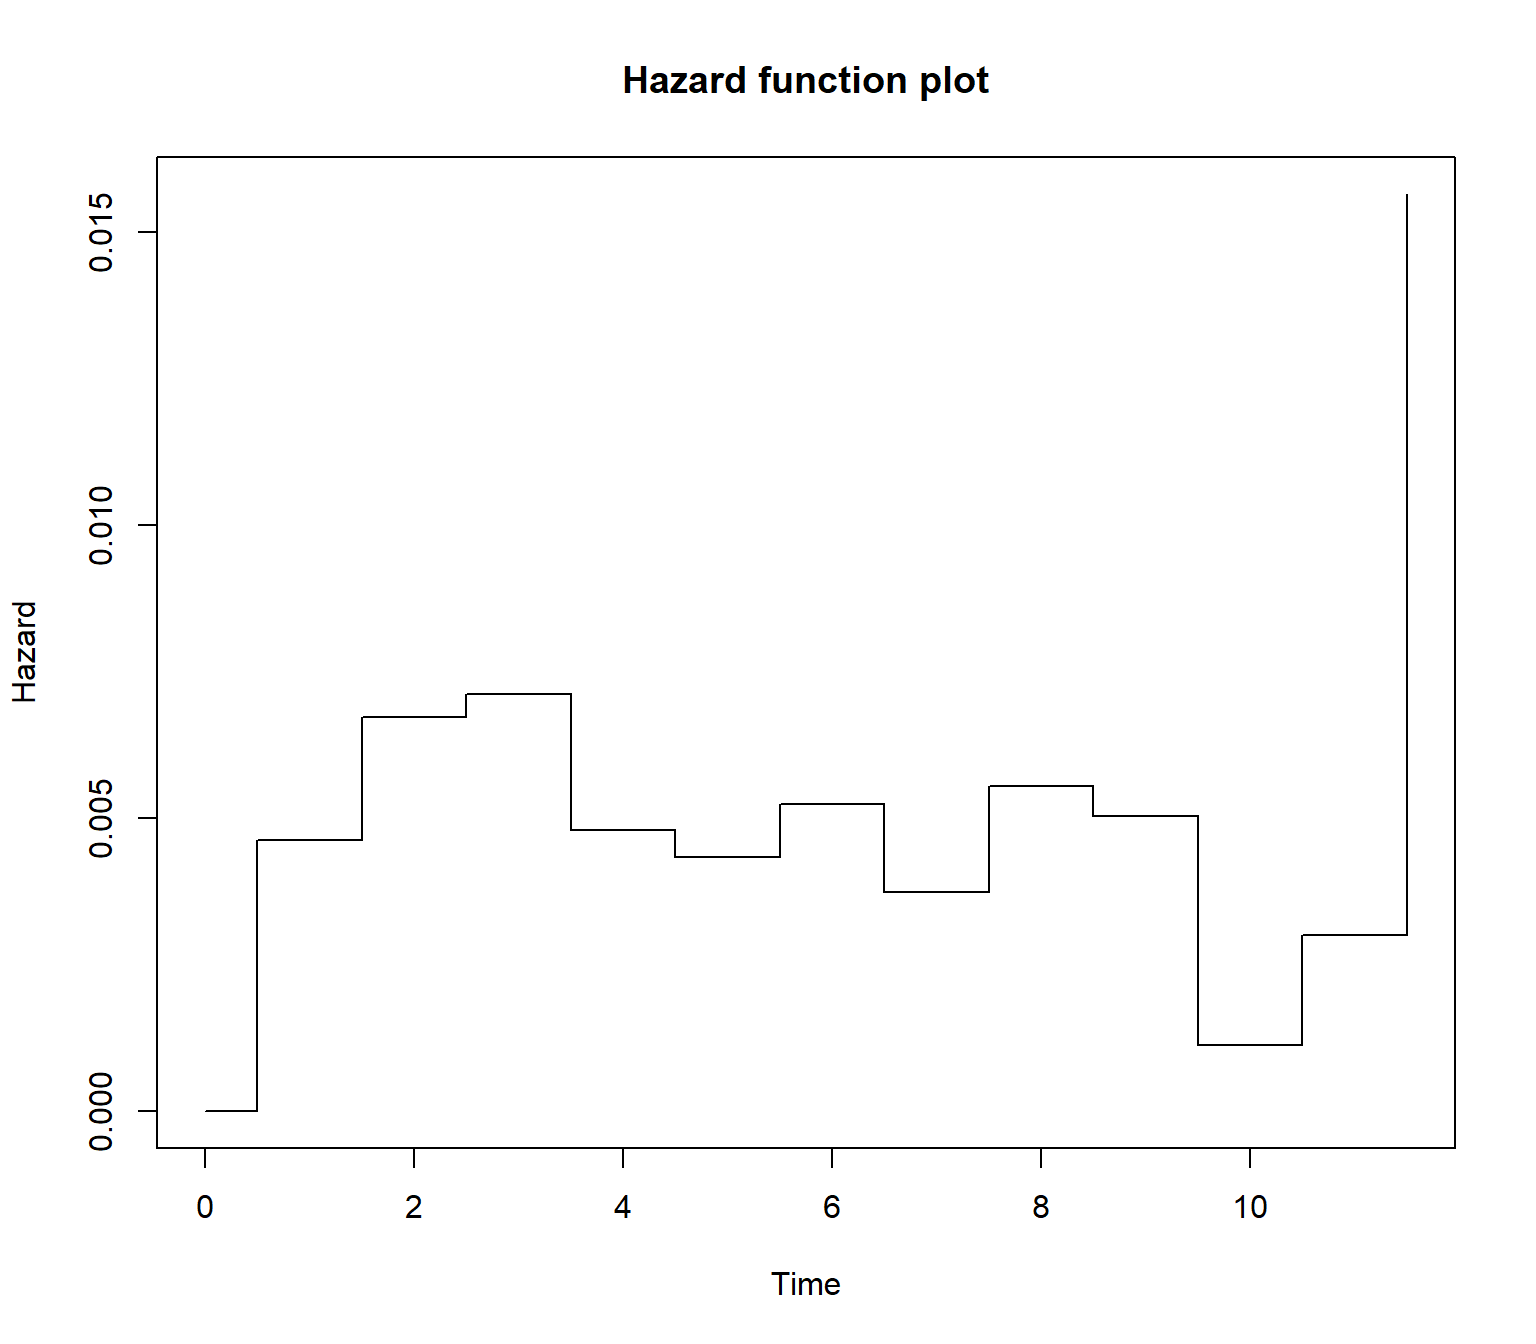
\includegraphics{EX3_Parametric_Hazard_Models_files/figure-latex/unnamed-chunk-13-1.pdf}

\begin{Shaded}
\begin{Highlighting}[]
\KeywordTok{plot}\NormalTok{(fit}\FloatTok{.5}\NormalTok{, }\DataTypeTok{fn=}\StringTok{"haz"}\NormalTok{, }\DataTypeTok{ylim=}\KeywordTok{c}\NormalTok{(}\DecValTok{0}\NormalTok{, }\FloatTok{.05}\NormalTok{))}
\KeywordTok{lines}\NormalTok{(fit.haz.sm, }\DataTypeTok{col=}\DecValTok{2}\NormalTok{)}
\end{Highlighting}
\end{Shaded}

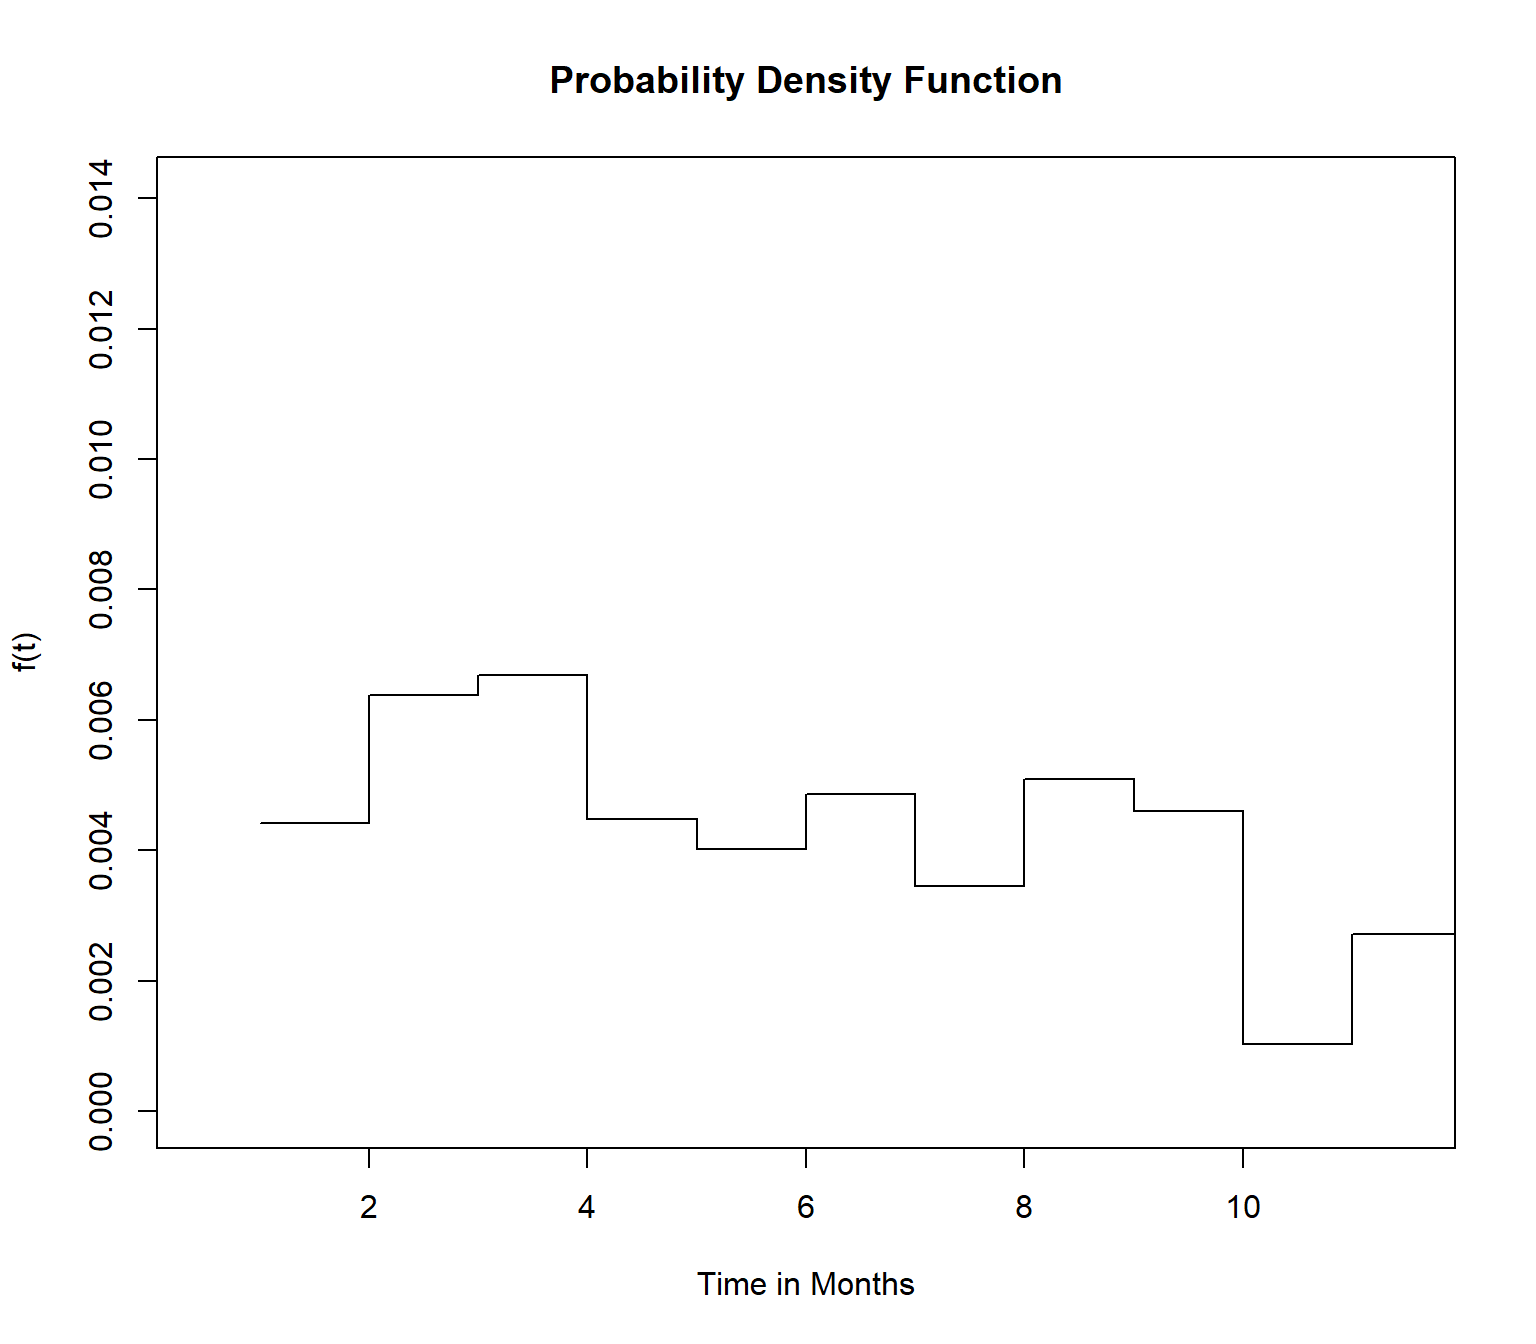
\includegraphics{EX3_Parametric_Hazard_Models_files/figure-latex/unnamed-chunk-13-2.pdf}

Which looks like it actually fits the data pretty good. The AIC's show
the log-logistic model still fitting better.

\begin{Shaded}
\begin{Highlighting}[]
\NormalTok{AIC5<-}\OperatorTok{-}\DecValTok{2}\OperatorTok{*}\NormalTok{fit}\FloatTok{.5}\OperatorTok{$}\NormalTok{loglik[}\DecValTok{2}\NormalTok{]}\OperatorTok{+}\DecValTok{2}\OperatorTok{*}\KeywordTok{length}\NormalTok{(fit}\FloatTok{.5}\OperatorTok{$}\NormalTok{coefficients); AIC5}
\end{Highlighting}
\end{Shaded}

\begin{verbatim}
## [1] 43397.15
\end{verbatim}

\begin{Shaded}
\begin{Highlighting}[]
\NormalTok{AIC4}
\end{Highlighting}
\end{Shaded}

\begin{verbatim}
## [1] 41082
\end{verbatim}

\hypertarget{graphical-checks-on-the-model-fit}{%
\subsection{Graphical checks on the model
fit}\label{graphical-checks-on-the-model-fit}}

The \texttt{eha} package also provides a graphical method for the
Cumulative hazard function, which allows us to visualize these models
even better. It uses the empirical hazard, as fit in the Cox model (more
on this next week), and compares the parametric models to the empirical
pattern:

\begin{Shaded}
\begin{Highlighting}[]
\NormalTok{emp<-}\KeywordTok{coxreg}\NormalTok{(}\KeywordTok{Surv}\NormalTok{(secbi, b2event)}\OperatorTok{~}\NormalTok{educ.high}\OperatorTok{+}\NormalTok{partnerhiedu}\OperatorTok{+}\KeywordTok{I}\NormalTok{(age}\OperatorTok{/}\DecValTok{5}\NormalTok{)}\OperatorTok{+}\NormalTok{age2,}
            \DataTypeTok{data=}\NormalTok{sub2[sub2}\OperatorTok{$}\NormalTok{secbi}\OperatorTok{>}\DecValTok{0}\NormalTok{,])}

\KeywordTok{check.dist}\NormalTok{(}\DataTypeTok{sp=}\NormalTok{emp,}\DataTypeTok{pp=}\NormalTok{fit}\FloatTok{.1}\NormalTok{, }\DataTypeTok{main =} \StringTok{"Empirical vs. Exponential"}\NormalTok{)}
\end{Highlighting}
\end{Shaded}

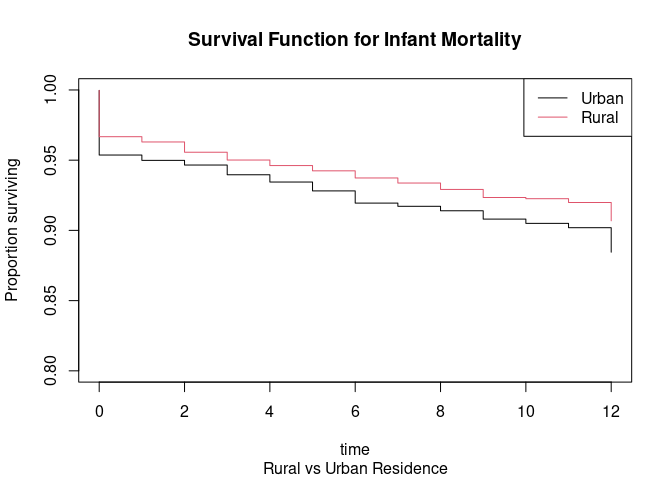
\includegraphics{EX3_Parametric_Hazard_Models_files/figure-latex/unnamed-chunk-15-1.pdf}

\begin{Shaded}
\begin{Highlighting}[]
\KeywordTok{check.dist}\NormalTok{(}\DataTypeTok{sp=}\NormalTok{emp,}\DataTypeTok{pp=}\NormalTok{fit}\FloatTok{.2}\NormalTok{, }\DataTypeTok{main =} \StringTok{"Empirical vs. Weibull"}\NormalTok{)}
\end{Highlighting}
\end{Shaded}

\includegraphics{EX3_Parametric_Hazard_Models_files/figure-latex/unnamed-chunk-15-2.pdf}

\begin{Shaded}
\begin{Highlighting}[]
\KeywordTok{check.dist}\NormalTok{(}\DataTypeTok{sp=}\NormalTok{emp,}\DataTypeTok{pp=}\NormalTok{fit}\FloatTok{.3}\NormalTok{, }\DataTypeTok{main =} \StringTok{"Empirical vs. Log-Normal"}\NormalTok{)}
\end{Highlighting}
\end{Shaded}

\includegraphics{EX3_Parametric_Hazard_Models_files/figure-latex/unnamed-chunk-15-3.pdf}

\begin{Shaded}
\begin{Highlighting}[]
\KeywordTok{check.dist}\NormalTok{(}\DataTypeTok{sp=}\NormalTok{emp,}\DataTypeTok{pp=}\NormalTok{fit}\FloatTok{.4}\NormalTok{, }\DataTypeTok{main =} \StringTok{"Empirical vs. Log-Logistic"}\NormalTok{)}
\end{Highlighting}
\end{Shaded}

\includegraphics{EX3_Parametric_Hazard_Models_files/figure-latex/unnamed-chunk-15-4.pdf}

\begin{Shaded}
\begin{Highlighting}[]
\KeywordTok{check.dist}\NormalTok{(}\DataTypeTok{sp=}\NormalTok{emp,}\DataTypeTok{pp=}\NormalTok{fit}\FloatTok{.5}\NormalTok{, }\DataTypeTok{main =} \StringTok{"Empirical vs. PCH"}\NormalTok{)}
\end{Highlighting}
\end{Shaded}

\includegraphics{EX3_Parametric_Hazard_Models_files/figure-latex/unnamed-chunk-15-5.pdf}

We see that the PCH model and the log-logistic models both appear to fit
the empirical hazard function better than the other parametric models.

\hypertarget{using-survey-design}{%
\subsection{Using Survey design}\label{using-survey-design}}

There are no survey analysis functions to fit parametric hazard models,
so we must roll our own using advice from Thomas Lumely in his book
\href{http://uq5sd9vt7m.search.serialssolutions.com/?ctx_ver=Z39.88-2004\&ctx_enc=info\%3Aofi\%2Fenc\%3AUTF-8\&rfr_id=info\%3Asid\%2Fsummon.serialssolutions.com\&rft_val_fmt=info\%3Aofi\%2Ffmt\%3Akev\%3Amtx\%3Abook\&rft.genre=book\&rft.title=Wiley+Series+in+Survey+Methodology\&rft.au=Lumley\%2C+Thomas\&rft.date=2010-03-11\&rft.pub=Wiley\&rft.isbn=9780470284308\&rft.externalDocID=10375602\&paramdict=en-US}{Appendix
E} \textbf{You can get this on campus through the library.}

\begin{Shaded}
\begin{Highlighting}[]
\NormalTok{survey.fit <-}\StringTok{ }\KeywordTok{withReplicates}\NormalTok{(rep.des, }
                             \KeywordTok{quote}\NormalTok{(}\KeywordTok{coef}\NormalTok{(}\KeywordTok{survreg}\NormalTok{(}\KeywordTok{Surv}\NormalTok{(secbi, b2event)}\OperatorTok{~}\NormalTok{educ.high}\OperatorTok{+}\NormalTok{partnerhiedu}\OperatorTok{+}\KeywordTok{I}\NormalTok{(age}\OperatorTok{/}\DecValTok{5}\NormalTok{)}\OperatorTok{+}\NormalTok{age2,}\DataTypeTok{dist=}\StringTok{"lognormal"}\NormalTok{, }\DataTypeTok{weights =}\NormalTok{ .weights}\FloatTok{+.0001}\NormalTok{))))}
\NormalTok{survey.est<-}\KeywordTok{as.data.frame}\NormalTok{(survey.fit)}
\NormalTok{survey.test<-}\KeywordTok{data.frame}\NormalTok{(}\DataTypeTok{beta =} \KeywordTok{rownames}\NormalTok{(survey.est), }\DataTypeTok{estimate=}\NormalTok{survey.est}\OperatorTok{$}\NormalTok{theta, }\DataTypeTok{se.est=}\NormalTok{ survey.est}\OperatorTok{$}\NormalTok{SE)}
\NormalTok{survey.test}\OperatorTok{$}\NormalTok{t<-survey.test}\OperatorTok{$}\NormalTok{estimate}\OperatorTok{/}\NormalTok{survey.test}\OperatorTok{$}\NormalTok{se.est}
\NormalTok{survey.test}\OperatorTok{$}\NormalTok{pval<-}\DecValTok{2}\OperatorTok{*}\KeywordTok{pnorm}\NormalTok{(survey.test}\OperatorTok{$}\NormalTok{t,}\DataTypeTok{lower.tail =}\NormalTok{ F )}
\NormalTok{survey.test}
\end{Highlighting}
\end{Shaded}

\begin{verbatim}
##           beta     estimate      se.est         t         pval
## 1  (Intercept)  3.385308441 0.051194252 66.126729 0.000000e+00
## 2    educ.high  0.221824182 0.033921853  6.539271 6.181953e-11
## 3 partnerhiedu  0.130191973 0.050823155  2.561667 1.041713e-02
## 4     I(age/5)  0.067808360 0.012338686  5.495590 3.894059e-08
## 5         age2 -0.004319788 0.001296868 -3.330939 1.999134e+00
\end{verbatim}

\begin{Shaded}
\begin{Highlighting}[]
\NormalTok{fit.}\FloatTok{2.}\NormalTok{aft<-}\KeywordTok{survreg}\NormalTok{(}\KeywordTok{Surv}\NormalTok{(secbi, b2event)}\OperatorTok{~}\NormalTok{educ.high}\OperatorTok{+}\NormalTok{partnerhiedu}\OperatorTok{+}\KeywordTok{I}\NormalTok{(age}\OperatorTok{/}\DecValTok{5}\NormalTok{)}\OperatorTok{+}\NormalTok{age2 }\OperatorTok{+}\StringTok{ }\NormalTok{age2, }\DataTypeTok{data=}\NormalTok{sub2[sub2}\OperatorTok{$}\NormalTok{secbi}\OperatorTok{>}\DecValTok{0}\NormalTok{,],}\DataTypeTok{dist =} \StringTok{"lognormal"}\NormalTok{)}

\NormalTok{fit.}\FloatTok{2.}\NormalTok{aft.sum<-}\KeywordTok{summary}\NormalTok{(fit.}\FloatTok{2.}\NormalTok{aft)}

\CommentTok{#Compare the se's of the parameters}
\NormalTok{survey.test}\OperatorTok{$}\NormalTok{se.est}\OperatorTok{/}\KeywordTok{sqrt}\NormalTok{(}\KeywordTok{diag}\NormalTok{(fit.}\FloatTok{2.}\NormalTok{aft.sum}\OperatorTok{$}\NormalTok{var[}\OperatorTok{-}\DecValTok{6}\NormalTok{, }\DecValTok{-6}\NormalTok{]))}
\end{Highlighting}
\end{Shaded}

\begin{verbatim}
## [1] 1.298721 1.323572 1.352203 1.422209 1.518569
\end{verbatim}

\begin{Shaded}
\begin{Highlighting}[]
\CommentTok{#survey based errors are larger, as they should be.}
\end{Highlighting}
\end{Shaded}

\hypertarget{using-longitudinal-data}{%
\subsection{Using Longitudinal Data}\label{using-longitudinal-data}}

As in the other examples, I illustrate fitting these models to data that
are longitudinal, instead of person-duration.

In this example, we will examine how to fit the parametric model to a
longitudinally collected data set. Here I use data from the
\href{http://nces.ed.gov/ecls/kinderdatainformation.asp}{ECLS-K}.
Specifically, we will examine the transition into poverty between
kindergarten and third grade.

First we load our data

\begin{Shaded}
\begin{Highlighting}[]
\NormalTok{eclskk5<-}\KeywordTok{readRDS}\NormalTok{(}\StringTok{"/mnt/c/Users/ozd504/OneDrive - University of Texas at San Antonio/classes/dem7223/dem7223_20//data/eclskk5.rds"}\NormalTok{)}
\KeywordTok{names}\NormalTok{(eclskk5)<-}\KeywordTok{tolower}\NormalTok{(}\KeywordTok{names}\NormalTok{(eclskk5))}
\CommentTok{#get out only the variables I'm going to use for this example}
\NormalTok{myvars<-}\KeywordTok{c}\NormalTok{( }\StringTok{"childid"}\NormalTok{,}\StringTok{"x_chsex_r"}\NormalTok{, }\StringTok{"x_raceth_r"}\NormalTok{, }\StringTok{"x1kage_r"}\NormalTok{,}\StringTok{"x4age"}\NormalTok{, }\StringTok{"x5age"}\NormalTok{, }\StringTok{"x6age"}\NormalTok{, }\StringTok{"x7age"}\NormalTok{, }\StringTok{"x2povty"}\NormalTok{,}\StringTok{"x4povty_i"}\NormalTok{, }\StringTok{"x6povty_i"}\NormalTok{, }\StringTok{"x8povty_i"}\NormalTok{,}\StringTok{"x12par1ed_i"}\NormalTok{, }\StringTok{"s2_id"}\NormalTok{, }\StringTok{"w6c6p_6psu"}\NormalTok{, }\StringTok{"w6c6p_6str"}\NormalTok{, }\StringTok{"w6c6p_20"}\NormalTok{)}
\NormalTok{eclskk5<-eclskk5[,myvars]}
\end{Highlighting}
\end{Shaded}

\begin{Shaded}
\begin{Highlighting}[]
\NormalTok{eclskk5}\OperatorTok{$}\NormalTok{age1<-}\KeywordTok{ifelse}\NormalTok{(eclskk5}\OperatorTok{$}\NormalTok{x1kage_r}\OperatorTok{==-}\DecValTok{9}\NormalTok{, }\OtherTok{NA}\NormalTok{, eclskk5}\OperatorTok{$}\NormalTok{x1kage_r}\OperatorTok{/}\DecValTok{12}\NormalTok{)}
\NormalTok{eclskk5}\OperatorTok{$}\NormalTok{age2<-}\KeywordTok{ifelse}\NormalTok{(eclskk5}\OperatorTok{$}\NormalTok{x4age}\OperatorTok{==-}\DecValTok{9}\NormalTok{, }\OtherTok{NA}\NormalTok{, eclskk5}\OperatorTok{$}\NormalTok{x4age}\OperatorTok{/}\DecValTok{12}\NormalTok{)}
\CommentTok{#for the later waves, the NCES group the ages into ranges of months, so 1= <105 months, 2=105 to 108 months. So, I fix the age at the midpoint of the interval they give, and make it into years by dividing by 12}
\NormalTok{eclskk5}\OperatorTok{$}\NormalTok{age3<-}\KeywordTok{ifelse}\NormalTok{(eclskk5}\OperatorTok{$}\NormalTok{x5age}\OperatorTok{==-}\DecValTok{9}\NormalTok{, }\OtherTok{NA}\NormalTok{, eclskk5}\OperatorTok{$}\NormalTok{x5age}\OperatorTok{/}\DecValTok{12}\NormalTok{)}

\NormalTok{eclskk5}\OperatorTok{$}\NormalTok{pov1<-}\KeywordTok{ifelse}\NormalTok{(eclskk5}\OperatorTok{$}\NormalTok{x2povty}\OperatorTok{==}\DecValTok{1}\NormalTok{,}\DecValTok{1}\NormalTok{,}\DecValTok{0}\NormalTok{)}
\NormalTok{eclskk5}\OperatorTok{$}\NormalTok{pov2<-}\KeywordTok{ifelse}\NormalTok{(eclskk5}\OperatorTok{$}\NormalTok{x4povty_i}\OperatorTok{==}\DecValTok{1}\NormalTok{,}\DecValTok{1}\NormalTok{,}\DecValTok{0}\NormalTok{)}
\NormalTok{eclskk5}\OperatorTok{$}\NormalTok{pov3<-}\KeywordTok{ifelse}\NormalTok{(eclskk5}\OperatorTok{$}\NormalTok{x6povty_i}\OperatorTok{==}\DecValTok{1}\NormalTok{,}\DecValTok{1}\NormalTok{,}\DecValTok{0}\NormalTok{)}

\CommentTok{#Recode race with white, non Hispanic as reference using dummy vars}
\NormalTok{eclskk5}\OperatorTok{$}\NormalTok{race_rec<-}\KeywordTok{Recode}\NormalTok{ (eclskk5}\OperatorTok{$}\NormalTok{x_raceth_r, }\DataTypeTok{recodes=}\StringTok{"1 = 'nhwhite';2='nhblack';3:4='hispanic';5='nhasian'; 6:8='other';-9=NA"}\NormalTok{, }\DataTypeTok{as.factor =}\NormalTok{ T)}
\NormalTok{eclskk5}\OperatorTok{$}\NormalTok{male<-}\KeywordTok{Recode}\NormalTok{(eclskk5}\OperatorTok{$}\NormalTok{x_chsex_r, }\DataTypeTok{recodes=}\StringTok{"1=1; 2=0; -9=NA"}\NormalTok{)}
\NormalTok{eclskk5}\OperatorTok{$}\NormalTok{mlths<-}\KeywordTok{Recode}\NormalTok{(eclskk5}\OperatorTok{$}\NormalTok{x12par1ed_i, }\DataTypeTok{recodes =} \StringTok{"1:2=1; 3:9=0; else = NA"}\NormalTok{)}
\NormalTok{eclskk5}\OperatorTok{$}\NormalTok{mgths<-}\KeywordTok{Recode}\NormalTok{(eclskk5}\OperatorTok{$}\NormalTok{x12par1ed_i, }\DataTypeTok{recodes =} \StringTok{"1:3=0; 4:9=1; else =NA"}\NormalTok{) }
\end{Highlighting}
\end{Shaded}

Now, I need to form the transition variable, this is my event variable,
and in this case it will be 1 if a child enters poverty between the
first wave of the data and the third grade wave, and 0 otherwise.

\textbf{NOTE} I need to remove any children who are already in poverty
age wave 1, because they are not at risk of experiencing \textbf{this
particular} transition. Again, this is called forming the \emph{risk
set}

\begin{Shaded}
\begin{Highlighting}[]
\NormalTok{eclskk5<-}\KeywordTok{subset}\NormalTok{(eclskk5, }\KeywordTok{is.na}\NormalTok{(pov1)}\OperatorTok{==}\NormalTok{F}\OperatorTok{&}\KeywordTok{is.na}\NormalTok{(pov2)}\OperatorTok{==}\NormalTok{F}\OperatorTok{&}\KeywordTok{is.na}\NormalTok{(pov3)}\OperatorTok{==}\NormalTok{F}\OperatorTok{&}\KeywordTok{is.na}\NormalTok{(age1)}\OperatorTok{==}\NormalTok{F}\OperatorTok{&}\KeywordTok{is.na}\NormalTok{(age2)}\OperatorTok{==}\NormalTok{F}\OperatorTok{&}\KeywordTok{is.na}\NormalTok{(age3)}\OperatorTok{==}\NormalTok{F}\OperatorTok{&}\NormalTok{pov1}\OperatorTok{!=}\DecValTok{1}\NormalTok{)}
\end{Highlighting}
\end{Shaded}

Now we do the entire data set. To analyze data longitudinally, we need
to reshape the data from the current ``wide'' format (repeated measures
in columns) to a ``long'' format (repeated observations in rows). The
\texttt{reshape()} function allows us to do this easily. It allows us to
specify our repeated measures, time varying covariates as well as
time-constant covariates.

\begin{Shaded}
\begin{Highlighting}[]
\NormalTok{e.long<-}\KeywordTok{reshape}\NormalTok{(}\KeywordTok{data.frame}\NormalTok{(eclskk5), }\DataTypeTok{idvar=}\StringTok{"childid"}\NormalTok{, }\DataTypeTok{varying=}\KeywordTok{list}\NormalTok{(}\KeywordTok{c}\NormalTok{(}\StringTok{"age1"}\NormalTok{,}\StringTok{"age2"}\NormalTok{),}
                                                     \KeywordTok{c}\NormalTok{(}\StringTok{"age2"}\NormalTok{, }\StringTok{"age3"}\NormalTok{)),}
                \DataTypeTok{v.names=}\KeywordTok{c}\NormalTok{(}\StringTok{"age_enter"}\NormalTok{, }\StringTok{"age_exit"}\NormalTok{),}
                \DataTypeTok{times=}\DecValTok{1}\OperatorTok{:}\DecValTok{2}\NormalTok{, }\DataTypeTok{direction=}\StringTok{"long"}\NormalTok{ )}
\NormalTok{e.long<-e.long[}\KeywordTok{order}\NormalTok{(e.long}\OperatorTok{$}\NormalTok{childid, e.long}\OperatorTok{$}\NormalTok{time),]}

\NormalTok{e.long}\OperatorTok{$}\NormalTok{povtran<-}\OtherTok{NA}

\NormalTok{e.long}\OperatorTok{$}\NormalTok{povtran[e.long}\OperatorTok{$}\NormalTok{pov1}\OperatorTok{==}\DecValTok{0}\OperatorTok{&}\NormalTok{e.long}\OperatorTok{$}\NormalTok{pov2}\OperatorTok{==}\DecValTok{1}\OperatorTok{&}\NormalTok{e.long}\OperatorTok{$}\NormalTok{time}\OperatorTok{==}\DecValTok{1}\NormalTok{]<-}\DecValTok{1}
\NormalTok{e.long}\OperatorTok{$}\NormalTok{povtran[e.long}\OperatorTok{$}\NormalTok{pov2}\OperatorTok{==}\DecValTok{0}\OperatorTok{&}\NormalTok{e.long}\OperatorTok{$}\NormalTok{pov3}\OperatorTok{==}\DecValTok{1}\OperatorTok{&}\NormalTok{e.long}\OperatorTok{$}\NormalTok{time}\OperatorTok{==}\DecValTok{2}\NormalTok{]<-}\DecValTok{1}

\NormalTok{e.long}\OperatorTok{$}\NormalTok{povtran[e.long}\OperatorTok{$}\NormalTok{pov1}\OperatorTok{==}\DecValTok{0}\OperatorTok{&}\NormalTok{e.long}\OperatorTok{$}\NormalTok{pov2}\OperatorTok{==}\DecValTok{0}\OperatorTok{&}\NormalTok{e.long}\OperatorTok{$}\NormalTok{time}\OperatorTok{==}\DecValTok{1}\NormalTok{]<-}\DecValTok{0}
\NormalTok{e.long}\OperatorTok{$}\NormalTok{povtran[e.long}\OperatorTok{$}\NormalTok{pov2}\OperatorTok{==}\DecValTok{0}\OperatorTok{&}\NormalTok{e.long}\OperatorTok{$}\NormalTok{pov3}\OperatorTok{==}\DecValTok{0}\OperatorTok{&}\NormalTok{e.long}\OperatorTok{$}\NormalTok{time}\OperatorTok{==}\DecValTok{2}\NormalTok{]<-}\DecValTok{0}

\CommentTok{#find which kids failed in earlier time periods and remove them from the second & third period risk set}
\NormalTok{failed1<-}\KeywordTok{which}\NormalTok{(}\KeywordTok{is.na}\NormalTok{(e.long}\OperatorTok{$}\NormalTok{povtran)}\OperatorTok{==}\NormalTok{T)}
\NormalTok{e.long<-e.long[}\OperatorTok{-}\NormalTok{failed1,]}


\NormalTok{e.long}\OperatorTok{$}\NormalTok{age1r<-}\KeywordTok{round}\NormalTok{(e.long}\OperatorTok{$}\NormalTok{age_enter, }\DecValTok{0}\NormalTok{)}
\NormalTok{e.long}\OperatorTok{$}\NormalTok{age2r<-}\KeywordTok{round}\NormalTok{(e.long}\OperatorTok{$}\NormalTok{age_exit, }\DecValTok{0}\NormalTok{)}
\KeywordTok{head}\NormalTok{(e.long, }\DataTypeTok{n=}\DecValTok{10}\NormalTok{)}
\end{Highlighting}
\end{Shaded}

\begin{verbatim}
##             childid x_chsex_r x_raceth_r x1kage_r x4age x5age  x6age  x7age
## 10000014.1 10000014         1          1    67.82 85.94 91.73  97.51 106.85
## 10000014.2 10000014         1          1    67.82 85.94 91.73  97.51 106.85
## 10000020.1 10000020         2          5    68.38 88.57 93.37 100.34 111.12
## 10000020.2 10000020         2          5    68.38 88.57 93.37 100.34 111.12
## 10000022.1 10000022         2          8    68.61 87.68 92.98  99.19 110.99
## 10000022.2 10000022         2          8    68.61 87.68 92.98  99.19 110.99
## 10000029.1 10000029         2          1    69.40 86.86 92.68  99.32 110.40
## 10000029.2 10000029         2          1    69.40 86.86 92.68  99.32 110.40
## 10000034.1 10000034         1          2    76.24 93.30 99.55 105.96 115.10
## 10000034.2 10000034         1          2    76.24 93.30 99.55 105.96 115.10
##            x2povty x4povty_i x6povty_i x8povty_i x12par1ed_i s2_id w6c6p_6psu
## 10000014.1       3         3         3         3           3  1433          2
## 10000014.2       3         3         3         3           3  1433          2
## 10000020.1       3         3         3         3           3  1365          2
## 10000020.2       3         3         3         3           3  1365          2
## 10000022.1       3         3         3         3           6  1405          1
## 10000022.2       3         3         3         3           6  1405          1
## 10000029.1       2         2         2         2           1  2042          2
## 10000029.2       2         2         2         2           1  2042          2
## 10000034.1       2         2         1        NA           3  2008          1
## 10000034.2       2         2         1        NA           3  2008          1
##            w6c6p_6str w6c6p_20 pov1 pov2 pov3 race_rec male mlths mgths time
## 10000014.1         39 328.0577    0    0    0  nhwhite    1     0     0    1
## 10000014.2         39 328.0577    0    0    0  nhwhite    1     0     0    2
## 10000020.1         53 136.5265    0    0    0  nhasian    0     0     0    1
## 10000020.2         53 136.5265    0    0    0  nhasian    0     0     0    2
## 10000022.1         35 163.1234    0    0    0    other    0     0     1    1
## 10000022.2         35 163.1234    0    0    0    other    0     0     1    2
## 10000029.1         60 341.5456    0    0    0  nhwhite    0     1     0    1
## 10000029.2         60 341.5456    0    0    0  nhwhite    0     1     0    2
## 10000034.1         50 289.4607    0    0    1  nhblack    1     0     0    1
## 10000034.2         50 289.4607    0    0    1  nhblack    1     0     0    2
##            age_enter age_exit povtran age1r age2r
## 10000014.1  5.651667 7.161667       0     6     7
## 10000014.2  7.161667 7.644167       0     7     8
## 10000020.1  5.698333 7.380833       0     6     7
## 10000020.2  7.380833 7.780833       0     7     8
## 10000022.1  5.717500 7.306667       0     6     7
## 10000022.2  7.306667 7.748333       0     7     8
## 10000029.1  5.783333 7.238333       0     6     7
## 10000029.2  7.238333 7.723333       0     7     8
## 10000034.1  6.353333 7.775000       0     6     8
## 10000034.2  7.775000 8.295833       1     8     8
\end{verbatim}

So, this shows us the repeated measures nature of the longitudinal data
set.

\begin{Shaded}
\begin{Highlighting}[]
\KeywordTok{library}\NormalTok{(survminer)}
\end{Highlighting}
\end{Shaded}

\begin{verbatim}
## Loading required package: ggplot2
\end{verbatim}

\begin{verbatim}
## Loading required package: ggpubr
\end{verbatim}

\begin{Shaded}
\begin{Highlighting}[]
\CommentTok{#poverty transition based on mother's education at time 1.}
\NormalTok{fit<-}\KeywordTok{survfit}\NormalTok{(}\KeywordTok{Surv}\NormalTok{(}\DataTypeTok{time =}\NormalTok{ time, }\DataTypeTok{event =}\NormalTok{ povtran)}\OperatorTok{~}\NormalTok{mlths, e.long)}
\KeywordTok{summary}\NormalTok{(fit)}
\end{Highlighting}
\end{Shaded}

\begin{verbatim}
## Call: survfit(formula = Surv(time = time, event = povtran) ~ mlths, 
##     data = e.long)
## 
## 9 observations deleted due to missingness 
##                 mlths=0 
##  time n.risk n.event survival std.err lower 95% CI upper 95% CI
##     1   3774     114     0.97 0.00279        0.964        0.975
##     2   1830      56     0.94 0.00475        0.931        0.949
## 
##                 mlths=1 
##  time n.risk n.event survival std.err lower 95% CI upper 95% CI
##     1    212      34     0.84  0.0252        0.792        0.891
##     2     89      19     0.66  0.0415        0.584        0.747
\end{verbatim}

\begin{Shaded}
\begin{Highlighting}[]
\KeywordTok{ggsurvplot}\NormalTok{(fit,}\DataTypeTok{conf.int =}\NormalTok{ T, }\DataTypeTok{risk.table =}\NormalTok{ F, }\DataTypeTok{title =} \StringTok{"Survivorship Function for Poverty Transition"}\NormalTok{, }\DataTypeTok{xlab =} \StringTok{"Wave of survey"}\NormalTok{)}
\end{Highlighting}
\end{Shaded}

\includegraphics{EX3_Parametric_Hazard_Models_files/figure-latex/unnamed-chunk-21-1.pdf}

Now we fit the models, I only show the Exponential, Weibull and PCH
model fit here, but the others follow the example from above. I specify
the age of the transition using an interval-censored notation to show
when a child began and ended each risk period.

\begin{Shaded}
\begin{Highlighting}[]
\CommentTok{#Exponential}
\CommentTok{#interval censored}
\NormalTok{fitl1<-}\KeywordTok{phreg}\NormalTok{(}\KeywordTok{Surv}\NormalTok{(}\DataTypeTok{time =}\NormalTok{ time, }\DataTypeTok{event =}\NormalTok{ povtran)}\OperatorTok{~}\NormalTok{mlths}\OperatorTok{+}\NormalTok{mgths}\OperatorTok{+}\NormalTok{race_rec, }\DataTypeTok{data=}\NormalTok{e.long, }\DataTypeTok{dist =} \StringTok{"weibull"}\NormalTok{, }\DataTypeTok{shape=}\DecValTok{1}\NormalTok{)}
\KeywordTok{summary}\NormalTok{(fitl1)  }
\end{Highlighting}
\end{Shaded}

\begin{verbatim}
## Call:
## phreg(formula = Surv(time = time, event = povtran) ~ mlths + 
##     mgths + race_rec, data = e.long, dist = "weibull", shape = 1)
## 
## Covariate          W.mean      Coef Exp(Coef)  se(Coef)    Wald p
## mlths               0.051     0.464     1.591     0.188     0.013 
## mgths               0.797    -1.178     0.308     0.160     0.000 
## race_rec 
##         hispanic    0.213     0         1           (reference)
##          nhasian    0.085    -0.655     0.519     0.291     0.024 
##          nhblack    0.063     0.004     1.004     0.242     0.986 
##          nhwhite    0.568    -1.097     0.334     0.179     0.000 
##            other    0.071    -0.338     0.713     0.286     0.236 
## 
## log(scale)                    2.072               0.136     0.000 
## 
##  Shape is fixed at  1 
## 
## Events                    223 
## Total time at risk          5905 
## Max. log. likelihood      -849.1 
## LR test statistic         209.06 
## Degrees of freedom        6 
## Overall p-value           0
\end{verbatim}

\begin{Shaded}
\begin{Highlighting}[]
\CommentTok{#Weibull}
\NormalTok{fitl2<-}\KeywordTok{phreg}\NormalTok{(}\KeywordTok{Surv}\NormalTok{(}\DataTypeTok{time =}\NormalTok{ time, }\DataTypeTok{event =}\NormalTok{ povtran)}\OperatorTok{~}\NormalTok{mlths}\OperatorTok{+}\NormalTok{mgths}\OperatorTok{+}\NormalTok{race_rec, }\DataTypeTok{data=}\NormalTok{e.long, }\DataTypeTok{dist =} \StringTok{"weibull"}\NormalTok{)}
\KeywordTok{summary}\NormalTok{(fitl2)  }
\end{Highlighting}
\end{Shaded}

\begin{verbatim}
## Call:
## phreg(formula = Surv(time = time, event = povtran) ~ mlths + 
##     mgths + race_rec, data = e.long, dist = "weibull")
## 
## Covariate          W.mean      Coef Exp(Coef)  se(Coef)    Wald p
## mlths               0.051     0.495     1.641     0.188     0.009 
## mgths               0.797    -1.197     0.302     0.160     0.000 
## race_rec 
##         hispanic    0.213     0         1           (reference)
##          nhasian    0.085    -0.657     0.518     0.291     0.024 
##          nhblack    0.063     0.007     1.007     0.243     0.978 
##          nhwhite    0.568    -1.112     0.329     0.179     0.000 
##            other    0.071    -0.350     0.705     0.286     0.221 
## 
## log(scale)                    1.077               0.056     0.000 
## log(shape)                    1.024               0.055     0.000 
## 
## Events                    223 
## Total time at risk          5905 
## Max. log. likelihood      -735.96 
## LR test statistic         217.30 
## Degrees of freedom        6 
## Overall p-value           0
\end{verbatim}

\begin{Shaded}
\begin{Highlighting}[]
\CommentTok{#Piecewise constant}
\NormalTok{fitl3<-}\KeywordTok{phreg}\NormalTok{(}\KeywordTok{Surv}\NormalTok{(}\DataTypeTok{time =}\NormalTok{ time, }\DataTypeTok{event =}\NormalTok{ povtran)}\OperatorTok{~}\NormalTok{mlths}\OperatorTok{+}\NormalTok{mgths}\OperatorTok{+}\NormalTok{race_rec,}\DataTypeTok{data=}\NormalTok{e.long, }\DataTypeTok{dist =} \StringTok{"pch"}\NormalTok{, }\DataTypeTok{cuts=}\KeywordTok{c}\NormalTok{(}\DecValTok{1}\NormalTok{))}
\KeywordTok{summary}\NormalTok{(fitl3)  }
\end{Highlighting}
\end{Shaded}

\begin{verbatim}
## Call:
## phreg(formula = Surv(time = time, event = povtran) ~ mlths + 
##     mgths + race_rec, data = e.long, dist = "pch", cuts = c(1))
## 
## Covariate          W.mean      Coef Exp(Coef)  se(Coef)    Wald p
## mlths               0.051     0.466     1.594     0.188     0.013 
## mgths               0.797    -1.179     0.308     0.160     0.000 
## race_rec 
##         hispanic    0.213     0         1           (reference)
##          nhasian    0.085    -0.655     0.519     0.291     0.024 
##          nhblack    0.063     0.004     1.004     0.242     0.986 
##          nhwhite    0.568    -1.097     0.334     0.179     0.000 
##            other    0.071    -0.339     0.712     0.286     0.235 
## 
## 
## Events                    223 
## Total time at risk          5905 
## Max. log. likelihood      -848.88 
## LR test statistic         209.38 
## Degrees of freedom        6 
## Overall p-value           0
\end{verbatim}

\begin{Shaded}
\begin{Highlighting}[]
\CommentTok{#AIC for exponential}
\DecValTok{-2}\OperatorTok{*}\NormalTok{fitl1}\OperatorTok{$}\NormalTok{loglik[}\DecValTok{2}\NormalTok{]}\OperatorTok{+}\DecValTok{2}\OperatorTok{*}\KeywordTok{length}\NormalTok{(fitl1}\OperatorTok{$}\NormalTok{coefficients)}
\end{Highlighting}
\end{Shaded}

\begin{verbatim}
## [1] 1712.204
\end{verbatim}

\begin{Shaded}
\begin{Highlighting}[]
\CommentTok{#AIC for weibull}
\DecValTok{-2}\OperatorTok{*}\NormalTok{fitl2}\OperatorTok{$}\NormalTok{loglik[}\DecValTok{2}\NormalTok{]}\OperatorTok{+}\DecValTok{2}\OperatorTok{*}\KeywordTok{length}\NormalTok{(fitl2}\OperatorTok{$}\NormalTok{coefficients)}
\end{Highlighting}
\end{Shaded}

\begin{verbatim}
## [1] 1487.925
\end{verbatim}

\begin{Shaded}
\begin{Highlighting}[]
\CommentTok{#AIC for weibull}
\DecValTok{-2}\OperatorTok{*}\NormalTok{fitl3}\OperatorTok{$}\NormalTok{loglik[}\DecValTok{2}\NormalTok{]}\OperatorTok{+}\DecValTok{2}\OperatorTok{*}\KeywordTok{length}\NormalTok{(fitl3}\OperatorTok{$}\NormalTok{coefficients)}
\end{Highlighting}
\end{Shaded}

\begin{verbatim}
## [1] 1709.755
\end{verbatim}

\begin{Shaded}
\begin{Highlighting}[]
\CommentTok{#Empirical (Cox)}
\NormalTok{fitle<-}\KeywordTok{coxreg}\NormalTok{(}\KeywordTok{Surv}\NormalTok{(}\DataTypeTok{time =}\NormalTok{ time, }\DataTypeTok{event =}\NormalTok{ povtran)}\OperatorTok{~}\NormalTok{mlths}\OperatorTok{+}\NormalTok{mgths}\OperatorTok{+}\NormalTok{race_rec, }\DataTypeTok{data=}\NormalTok{e.long)}

\KeywordTok{check.dist}\NormalTok{(fitle, fitl1, }\DataTypeTok{main =} \StringTok{"Exponential"}\NormalTok{)}
\end{Highlighting}
\end{Shaded}

\includegraphics{EX3_Parametric_Hazard_Models_files/figure-latex/unnamed-chunk-22-1.pdf}

\begin{Shaded}
\begin{Highlighting}[]
\KeywordTok{check.dist}\NormalTok{(fitle, fitl2, }\DataTypeTok{main =} \StringTok{"Weibull"}\NormalTok{)}
\end{Highlighting}
\end{Shaded}

\includegraphics{EX3_Parametric_Hazard_Models_files/figure-latex/unnamed-chunk-22-2.pdf}

\begin{Shaded}
\begin{Highlighting}[]
\KeywordTok{check.dist}\NormalTok{(fitle, fitl3, }\DataTypeTok{main =} \StringTok{"Piecewise Exponential"}\NormalTok{)}
\end{Highlighting}
\end{Shaded}

\includegraphics{EX3_Parametric_Hazard_Models_files/figure-latex/unnamed-chunk-22-3.pdf}

According to the AIC, the Weibull model is fitting better here.

\end{document}
